\documentclass[conference]{IEEEtran}
\usepackage[T1]{fontenc}
\usepackage[utf8]{inputenc}
\usepackage{microtype}
\usepackage{amsmath,amssymb,amsfonts}
\usepackage{algorithm}
\usepackage{algpseudocode}
\usepackage{graphicx}
\usepackage{xcolor}
\usepackage{booktabs}
\usepackage{multirow}
\usepackage{tabularx}
\usepackage{array}
\usepackage{url}
\usepackage{cite}
\usepackage{pifont}
\usepackage{hyperref}
\usepackage{tikz}
\usetikzlibrary{shapes.geometric, arrows.meta, positioning, fit, calc}
\usepackage{pgfplots}
\pgfplotsset{compat=1.18}
\usepackage{caption}
\usepackage{subcaption}
\usepackage{placeins}

\hypersetup{colorlinks=true,linkcolor=blue,citecolor=blue,urlcolor=blue}

\tikzset{
  block/.style={rectangle,rounded corners=4pt,draw=black!70,fill=blue!10,
    text width=4.0em,text centered,minimum height=2.0em,font=\scriptsize},
  wideblock/.style={rectangle,rounded corners=4pt,draw=black!70,fill=green!12,
    text width=6.0em,text centered,minimum height=2.0em,font=\scriptsize},
  decision/.style={diamond,draw=black!70,fill=orange!20,aspect=2.5,
    text width=3.8em,text centered,minimum height=1.5em,font=\scriptsize},
  llmblock/.style={rectangle,rounded corners=4pt,draw=black!70,fill=purple!12,
    text width=5.0em,text centered,minimum height=2.0em,font=\scriptsize},
  arrow/.style={-Stealth,thick,draw=black!70},
  dasharrow/.style={-Stealth,thick,dashed,draw=gray!70},
  startend/.style={rectangle,rounded corners=8pt,draw=black!80,fill=gray!20,
    text width=4.8em,text centered,minimum height=1.8em,font=\scriptsize}
}

\begin{document}

\title{AsanaAI: A Dual-Model Hybrid Architecture for\\
Real-Time Yoga Posture Correction with Occlusion Recovery\\
and LLM-Guided Safety Feedback}

\author{
\IEEEauthorblockN{Anamitra Sarkar}
\IEEEauthorblockA{\textit{Dept. of CSE (AI/ML)}\\
\textit{RCC Institute of Information Technology}\\
Kolkata, West Bengal, India}
\and
\IEEEauthorblockN{Debjit Deb Barman}
\IEEEauthorblockA{\textit{Dept. of CSE (AI/ML)}\\
\textit{RCC Institute of Information Technology}\\
Kolkata, West Bengal, India}
\and
\IEEEauthorblockN{Adrija Ray Mondal}
\IEEEauthorblockA{\textit{Dept. of CSE (AI/ML)}\\
\textit{RCC Institute of Information Technology}\\
Kolkata, West Bengal, India}
\and
\IEEEauthorblockN{Tanima Samanta}
\IEEEauthorblockA{\textit{Dept. of CSE (AI/ML)}\\
\textit{RCC Institute of Information Technology}\\
Kolkata, West Bengal, India}
\and
\IEEEauthorblockN{Sujit Chakraborty \textit{(Supervisor)}}
\IEEEauthorblockA{\textit{Assistant Professor, CSE}\\
\textit{RCC Institute of Information Technology}\\
Kolkata, West Bengal, India}
}

\maketitle

\begin{abstract}
Unsupervised yoga practice is a leading cause of preventable musculoskeletal injury,
motivating the need for an automated system that can supervise form with the reliability
of a human instructor on ordinary consumer hardware. Real-time automated yoga posture
correction presents a multi-dimensional challenge at the intersection of computer vision,
biomechanical signal processing, and safe human-computer interaction. Existing systems
predominantly rely on static frame-level classification, failing to capture dynamic
transitions between postures or adapt to user-specific anatomical constraints. This paper
presents \textbf{AsanaAI}, a production-grade dual-model hybrid system for real-time yoga
posture correction deployed as a Progressive Web Application. We adopt this dual-stream
design--pairing a lightweight residual MLP for instantaneous static-frame form checking
with a spatio-temporal graph convolutional network for motion-aware transition
analysis--specifically because a single frame-level classifier can judge alignment but
not movement trajectory, whereas the two together capture both while remaining cheap
enough for CPU-only deployment. Our architecture fuses two complementary streams:
(i) a \textbf{3-Head Residual MLP} that simultaneously predicts pose identity (23 classes,
93.38\% accuracy), binary correctness (96.81\% accuracy), and a 15-joint angle deviation
vector from a single 15-dimensional biomechanical feature frame; and (ii) a
\textbf{Spatio-Temporal Graph Convolutional Network (ST-GCN) Sequence
Classifier} processing 60-frame temporal windows of 99-dimensional pelvis-centered skeletal
coordinates (75.25\% accuracy). A confidence-gated cooperative pipeline selects the
appropriate stream per inference step. A symmetric kinematic occlusion recovery solver
mitigates self-occlusion artifacts. A \textbf{Digital Twin} calibration module personalizes
joint limits per user. A three-stage \textbf{LLM safety pipeline} (symbolic rules
$\rightarrow$ Groq-hosted Qwen-3.6-27B paraphrase $\rightarrow$ post-generation safety screening)
generates multilingual (English, Hindi, Bengali) voiced corrections without injury risk.
The full system achieves end-to-end latency under 500\,ms on CPU-only deployment within a
4\,GB RAM budget and is containerized for Hugging Face Spaces.
\end{abstract}

\begin{IEEEkeywords}
Yoga Posture Classification, Residual MLP, ST-GCN, MediaPipe,
Occlusion Recovery, Digital Twin Calibration, LLM Safety Pipeline, Multilingual
Voice Feedback, Progressive Web App, Real-Time Posture Correction
\end{IEEEkeywords}

%% =================================================================
\section{Introduction}
\label{sec:intro}
%% =================================================================

Yoga is practiced by over 300 million people worldwide as a holistic discipline targeting
physical health, mental wellbeing, and musculoskeletal flexibility~\cite{yoga_global_2024}.
Incorrect posture during practice is cited as the leading cause of yoga-related injuries,
particularly to the lower back, knees, and neck~\cite{injury_yoga_2022}. Professional
instructor supervision is rarely scalable to remote or resource-constrained practitioners.

Google's MediaPipe Pose Landmarker~\cite{mediapipe_2020} has enabled camera-based posture
feedback on commodity hardware without GPU accelerators. However, translating raw skeletal
landmark data into safe, actionable, personalized corrections remains an open research
problem. Existing automated systems such as YogAI~\cite{yogai2021} perform frame-level
keypoint comparison, ignoring temporal motion context, anatomical variation, and safety
constraints.

Several concrete research gaps motivate our design. First, most existing systems, such as
YogAI~\cite{yogai2021}, classify single frames in isolation,
leaving postural transitions unmodeled; temporal sequence modeling is needed to capture
these dynamics unavailable to frame-level classifiers. Second, prior pipelines discard or
misclassify frames with low-confidence joints arising from self-occlusion, a limitation
that volumetric mesh estimators such as CLIFF~\cite{cliff2022} address only at a GPU cost
unsuitable for our CPU-only target; we instead propose a symmetric kinematic solver for
robust joint recovery without additional sensors. Third, uniform correction thresholds,
such as the fixed angle-deviation rules of Liao et al.~\cite{action_correction_2020},
ignore anatomical variation across practitioners and produce false-positive correction
alerts; our Digital Twin calibration module eliminates this by personalizing joint ranges
per user. Fourth, unconstrained large language models risk hallucinating injury-causing
instructions when applied to exercise coaching~\cite{llm_fitness_2024}; our three-stage
safety pipeline bounds generation strictly to physiotherapist-validated corrections.
Finally, high-accuracy pose estimators such as HRNet~\cite{hrnet2019} and
ViTPose~\cite{vitpose2022} require continuous GPU inference, which is impractical for
low-bandwidth or resource-constrained deployments; our complete model footprint of under
300\,KB runs on a single CPU thread.

\medskip
\noindent\textbf{Contributions:}
\begin{itemize}
\item A novel \textbf{3-Head Residual MLP} performing simultaneous pose ID classification,
  correctness scoring, and joint deviation regression on a compact 15-angle feature vector.
\item A \textbf{Spatio-Temporal Graph Convolutional Network (ST-GCN)} sequence model with pelvis-centered
  scale normalization operating on 60-frame coordinate windows.
\item A \textbf{cooperative dual-stream pipeline} with a confidence-gated fallback mechanism.
\item A \textbf{symmetric kinematic occlusion recovery} algorithm.
\item A \textbf{Digital Twin} user-calibration module suppressing false correction alerts.
\item A \textbf{three-stage LLM safety pipeline} guaranteeing injury-free multilingual feedback.
\item A complete \textbf{open-source implementation} containerized in Docker and deployed
  on Hugging Face Spaces, with a Next.js TypeScript PWA frontend.
\end{itemize}

%% =================================================================
\section{Related Work}
\label{sec:related}
%% =================================================================

Each subsection below follows the same structure per work cited: what it
contributes, what we adopted or built on directly, and what gap it left open
that either motivated a design choice in this paper or remains an acknowledged
limitation of our own system.

\subsection{Pose Estimation Foundations}

\textbf{OpenPose~\cite{openpose2019}} introduced Part Affinity Fields for
multi-person 2D keypoint detection. \emph{Adopted:} its part-affinity concept
established that limb-connectivity, not just per-joint confidence, matters for
robust skeleton extraction, which motivated our own use of a fixed skeletal
adjacency graph (Table~\ref{tab:features}, Section~\ref{sec:sequence}).
\emph{Gap:} its multi-person design requires GPU inference, incompatible with
our free-tier CPU deployment target, so we did not use OpenPose itself.

\textbf{MediaPipe/BlazePose~\cite{mediapipe_2020}} provides 33 3D landmark
coordinates with visibility confidence at $<$15\,ms/frame on mobile CPU.
\emph{Adopted directly:} this is the landmark extractor our entire pipeline is
built on (Section~\ref{sec:feature}). \emph{Gap, discovered rather than
assumed:} the library's monocular $z$-depth output, while fast, is only
reliable at the camera framing consistency of continuous video capture; we
found (Section~\ref{sec:depth-limitation}) that this single limitation, not
model capacity, was the dominant cause of our real-world classification
failures --- a gap this paper diagnoses and partially mitigates rather than
one MediaPipe itself claims to solve.

\textbf{HRNet~\cite{hrnet2019} and ViTPose~\cite{vitpose2022}} achieve higher
keypoint accuracy than BlazePose through high-resolution and transformer-based
architectures respectively. \emph{Not adopted:} both require continuous GPU
inference (Section~\ref{sec:discussion-cost}), which is incompatible with the
near-zero-cost, free-tier hosting this system targets. \emph{Open question we
do not resolve:} whether either would have avoided the depth-reliability gap
above is untested here, since neither was integrated; Section~\ref{sec:future}
identifies a dedicated monocular 3D lifting model as the more targeted fix.

\subsection{Static Yoga Pose Classification}

\textbf{Yoga-82~\cite{yoga82_2021}} established a public benchmark of 82
fine-grained yoga poses. \emph{Adopted:} its hierarchical pose taxonomy
informed our own 23-class vocabulary design (Table~\ref{tab:poses}).
\emph{Gap we inherit, not solve:} Yoga-82 is an image-classification benchmark
with no live deployment or real-time constraint; our 35-image real-world
evaluation (Table~\ref{tab:depthablation}) suggests that strong accuracy on a
curated benchmark like Yoga-82 does not by itself guarantee reliability on
arbitrary user-captured photos, a gap this paper's live-testing methodology
was specifically designed to surface.

\textbf{Angle-based skeletal features~\cite{angle_yoga_2022}} showed that
biomechanical joint angles are more discriminative than raw coordinates for
pose classification. \emph{Adopted directly:} our entire 15-feature angle
representation (Table~\ref{tab:features}) follows this approach rather than
classifying on raw landmark coordinates. \emph{Gap this paper adds to:} that
prior work does not examine whether the 3D angle computation itself is robust
to camera-distance variation; our finding that it is not (absent the $z$
coordinate) is a direct, previously unreported extension of this line of work.

\textbf{Vision-transformer yoga classification~\cite{yogapose_transformer_2023}}
achieved strong fine-grained accuracy but requires high-resolution image
inputs processed through a full transformer backbone. \emph{Not adopted:}
incompatible with our lightweight, client-side keypoint extraction design.
\emph{Gap:} being image-based rather than skeleton-based, it is not directly
comparable to our real-world generalization findings, though the same
camera-framing sensitivity we identified would plausibly also affect any
image-input model trained on a narrow visual distribution.

\textbf{Skeleton-based robustness study~\cite{skeleton_yoga_2025}} showed
skeleton representations generalize better than raw image classification
across visual conditions. \emph{Adopted as motivation:} this supported our
skeleton-first design choice. \emph{Gap it did not anticipate:} that
generalization can still fail catastrophically when the skeleton's own $z$
coordinate is itself unreliable outside the training camera distribution ---
the central finding of Section~\ref{sec:depth-limitation} that this paper
contributes back to this literature.

\subsection{Temporal Sequence Analysis}

\textbf{ST-GCN~\cite{stgcn_2018}} pioneered graph convolutional networks over
skeleton joint adjacency for action recognition. \emph{Adopted directly:} our
sequence classifier (Section~\ref{sec:sequence}) is a direct architectural
descendant, using the same normalized adjacency convolution over MediaPipe's
33-joint graph. \emph{Gap:} ST-GCN targets generic action recognition (e.g.\
Kinetics-Skeleton), not the specific problem of distinguishing a held yoga
pose from an inter-pose transition; our label-construction and majority-vote
windowing (Section~\ref{sec:data}) address this but introduce their own
labeling-noise limitation (75.25\% vs.\ the MLP's 93.38\%, Table~\ref{tab:ablation}).

\textbf{PoseFormer~\cite{poseformer_2021}} applied spatio-temporal
transformers to 3D pose estimation. \emph{Not adopted:} transformer attention
over long sequences is heavier than our lightweight ST-GCN blocks warrant for
a CPU-only deployment target. \emph{Gap left for future work:} whether
attention-based temporal modeling would improve our 75.25\% sequence accuracy
is untested here.

\textbf{Pose-to-Pose~\cite{pose2pose_cvprw2025}} specifically identifies smooth
inter-pose transition modeling as an unsolved yoga-specific challenge.
\emph{Adopted as direct motivation:} this is precisely the gap our
\texttt{transition/unknown} class and Vinyasa-transition future work
(Section~\ref{sec:future}) target. \emph{Gap we still share with it:} neither
this paper nor Pose-to-Pose provides active corrective feedback \emph{during}
a transition, only during recognized static holds --- an explicitly
acknowledged open limitation (Section~\ref{sec:limitations}).

\textbf{GRU-based sequence models~\cite{gru_pose_2023}} showed lower-complexity
recurrent models can match transformer temporal accuracy at lower cost.
\emph{Considered but not adopted:} our ST-GCN block was chosen instead
specifically to exploit the fixed skeletal graph structure GRUs do not model
explicitly; a direct empirical comparison between the two on this dataset is
not performed here and would be a reasonable ablation for future work.

\subsection{Correction and Feedback Systems}

\textbf{Liao et al.~\cite{action_correction_2020}} proposed fixed angle-deviation
thresholding for exercise coaching feedback. \emph{Adopted and extended:} our
Stage-1 symbolic rule engine (Section~\ref{sec:llm}) generalizes this same
threshold-based principle across pose-specific joint templates in three
languages. \emph{Gap it left open, which we solve:} deviation thresholding
alone produces only fixed template text, with no natural-language variation;
our Stage 2--3 LLM paraphrase-and-safety-screen pipeline (Eq.~\ref{eq:safety})
adds natural language delivery while provably bounding it to the same
physiotherapist-approved template space.

\textbf{PosePilot~\cite{posepilot_2025}} explored edge-AI posture correction on
wearable hardware. \emph{Adopted as validation of the edge-deployment
philosophy:} it supports our own choice of client-side keypoint extraction
over server GPU inference. \emph{Gap it left open:} PosePilot's correction
output is derived directly from sensor thresholds with no conversational
guidance layer (Table~\ref{tab:comparison} marks it only ``Partial'' on temporal
modeling and \ding{55} on safety-bounded LLM feedback) --- the LLM safety
pipeline above is this paper's answer to that specific gap.

\textbf{LLM-based exercise coaching~\cite{llm_fitness_2024}} identified that
unconstrained LLM generation for fitness instructions risks hallucinating
unsafe guidance (e.g.\ ``push deeper''). \emph{Adopted directly as the problem
statement} motivating our entire Stage-3 forbidden-word safety screen
(Eq.~\ref{eq:safety}). \emph{Gap we do not fully close:} a keyword denylist is
a coarse, not semantic, safety filter --- a sufficiently paraphrased unsafe
instruction that avoids the exact forbidden tokens could still pass Stage 3
undetected; this is recorded as an open limitation rather than a solved
problem.

\textbf{YogAI~\cite{yogai2021}} performs frame-by-frame keypoint comparison
with no temporal modeling, occlusion handling, personalization, or
safety-bounded feedback. \emph{Used as the primary baseline comparison}
(Table~\ref{tab:comparison}) establishing the gap this entire system
architecture is designed to close --- its four compared columns map directly
onto our four major subsystems. \emph{Gap acknowledged in return:} our own
temporal accuracy (75.25\%) and real-world single-frame reliability
(Table~\ref{tab:depthablation}) are themselves imperfect, so the comparison is
one of architectural completeness, not a claim of uniformly superior raw
accuracy over every metric this simpler system reports. A generic multi-person
pose estimator such as PoseNet~\cite{posenet2019} was deliberately excluded
from this comparison rather than included as a weak baseline: it was never
designed as a yoga correction system at all, and comparing it on axes like
safety-bounded LLM feedback would not be a meaningful comparison in either
direction.

\textbf{CLIFF~\cite{cliff2022}} recovers full-body 3D mesh and location
information from a single image, capable of directly resolving occluded joint
positions via volumetric fitting. \emph{Adopted as an optional interface, not
implemented:} our fusion function (Section~\ref{sec:occlusion}) exposes a
pass-through slot for pre-computed CLIFF-style 3D coordinates, but our
free-tier CPU deployment does not bundle a CLIFF inference model --- CLIFF-style
volumetric fitting requires GPU inference incompatible with this system's
near-zero-cost hosting target. \emph{Gap we inherited rather than solved:}
production traffic always falls back to a lightweight symmetric
mirror-reflection heuristic (Eq.~\ref{eq:mirror}) instead, so full CLIFF-level
occlusion recovery is never active in the deployed system --- an explicit,
acknowledged limitation (Section~\ref{sec:limitations}), not a claim that our
occlusion recovery matches CLIFF's fidelity.

\subsection{Positioning}

Table~\ref{tab:comparison} summarizes this section's comparison quantitatively.
No prior work reviewed here combines temporal sequence modeling, occlusion
recovery, anatomical personalization, and safety-bounded LLM feedback in one
system; AsanaAI's contribution is this specific integration, evaluated
honestly against its own real-world failure modes (Section
\ref{sec:depth-limitation}) rather than only against in-distribution
benchmark numbers.

%% =================================================================
\section{System Architecture}
\label{sec:system}
%% =================================================================

\subsection{Overall Pipeline}

Fig.~\ref{fig:pipeline} illustrates the complete 13-stage processing pipeline. A live
camera frame is processed through MediaPipe, biomechanical features are extracted,
dual classifiers are applied, corrections are personalized via Digital Twin, and
spoken feedback is generated.

\begin{figure}[ht]
\centering
\scalebox{0.8}{
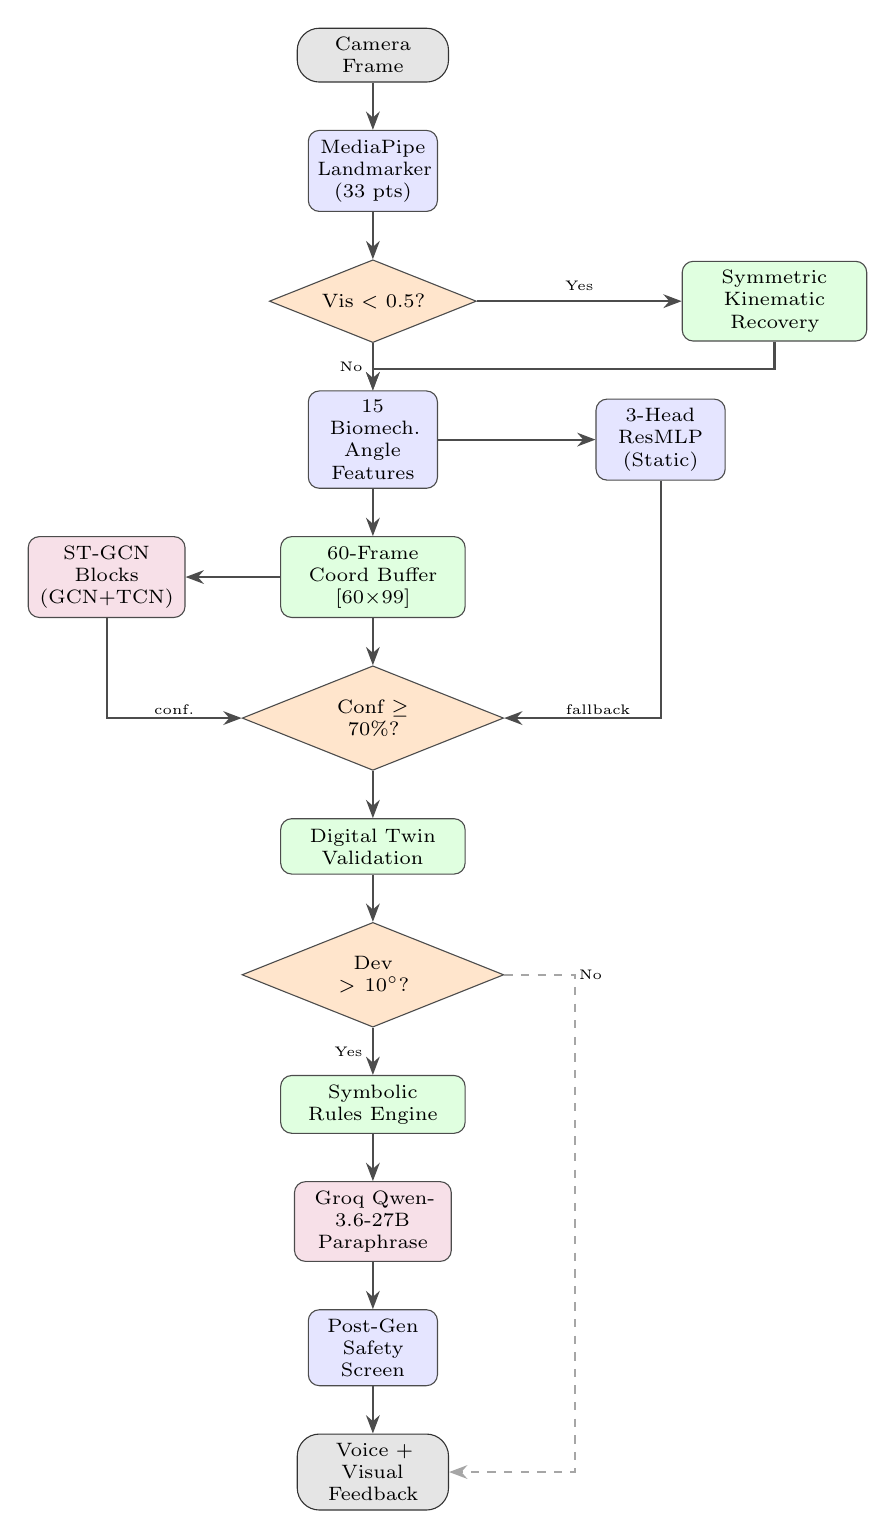
\begin{tikzpicture}[node distance=0.6cm and 0.5cm]
  \node[startend] (input) {Camera\\ Frame};
  \node[block, below=of input] (mp) {MediaPipe\\ Landmarker\\ (33 pts)};
  \node[decision, below=of mp] (occcheck) {Vis $<$ 0.5?};
  \node[wideblock, right=2.6cm of occcheck] (recover) {Symmetric\\ Kinematic\\ Recovery};
  \node[block, below=of occcheck] (angles) {15 Biomech.\\ Angle\\ Features};
  \node[wideblock, below=of angles] (buffer) {60-Frame\\ Coord Buffer\\ $[60{\times}99]$};
  \node[block, right=2.0cm of angles] (mlp) {3-Head\\ ResMLP\\ (Static)};
  \node[llmblock, left=1.2cm of buffer] (seq) {ST-GCN\\ Blocks\\ (GCN+TCN)};
  \node[decision, below=of buffer] (confgate) {Conf $\geq$ 70\%?};
  \node[wideblock, below=of confgate] (twin) {Digital Twin\\ Validation};
  \node[decision, below=of twin] (devcheck) {Dev $> 10^{\circ}$?};
  \node[wideblock, below=of devcheck] (sym) {Symbolic\\ Rules Engine};
  \node[llmblock, below=of sym] (groq) {Groq Qwen-\\ 3.6-27B\\ Paraphrase};
  \node[block, below=of groq] (safety) {Post-Gen\\ Safety Screen};
  \node[startend, below=of safety] (output) {Voice +\\ Visual\\ Feedback};

  \draw[arrow] (input) -- (mp);
  \draw[arrow] (mp) -- (occcheck);
  \draw[arrow] (occcheck) -- node[left,font=\tiny]{No} (angles);
  \draw[arrow] (occcheck) -- node[above,font=\tiny]{Yes} (recover);
  \draw[arrow] (recover.south) -- ++(0,-0.35) -| (angles.north);
  \draw[arrow] (angles) -- (buffer);
  \draw[arrow] (angles.east) -- (mlp.west);
  \draw[arrow] (buffer) -- (seq);
  \draw[arrow] (buffer) -- (confgate);
  \draw[arrow] (seq.south) |- node[above,font=\tiny,pos=0.75,fill=white,inner sep=1pt]{conf.} (confgate.west);
  \draw[arrow] (mlp.south) |- node[above,font=\tiny,pos=0.7,fill=white,inner sep=1pt]{fallback} (confgate.east);
  \draw[arrow] (confgate) -- (twin);
  \draw[arrow] (twin) -- (devcheck);
  \draw[arrow] (devcheck) -- node[left,font=\tiny]{Yes} (sym);
  \draw[dasharrow] (devcheck.east) -- ++(0.9,0)
    node[right,font=\tiny,fill=white,inner sep=1pt]{No} |- (output.east);
  \draw[arrow] (sym) -- (groq);
  \draw[arrow] (groq) -- (safety);
  \draw[arrow] (safety) -- (output);
\end{tikzpicture}
}
\caption{Complete 13-stage AsanaAI pipeline. Dual-model cooperative path:
sequence model (left) and static MLP (right) feed into a confidence gate,
then Digital Twin personalization, then LLM-guided feedback.}
\label{fig:pipeline}
\end{figure}

\subsection{Backend Modular Architecture}

The backend is implemented as a modular FastAPI service exposing REST endpoints for
frame-level pose analysis, sequence-level flow classification, correction generation,
and occlusion recovery. The two neural network architectures are defined independently
from the services that consume them: the sequence classifier's implementation class
retains a legacy name from an early development phase when a recurrent backbone was
planned, though the deployed architecture uses Spatio-Temporal Graph Convolutions
(Section~\ref{sec:sequence}). Trained model weights are fetched lazily and cached in
memory through a singleton loader backed by the Hugging Face Hub, avoiding repeated
downloads across requests. A dedicated occlusion-recovery service implements the
symmetric kinematic solver described in Section~\ref{sec:occlusion}, and a separate
correction-generation service implements the three-stage safety pipeline of
Section~\ref{sec:llm}. Angle computation and coordinate normalization are isolated in a
shared utility used by both classifiers. CPU threading is bounded to a single thread at
startup, keeping total RAM usage under 4\,GB.

\subsection{Frontend PWA Architecture}

The client is a Next.js TypeScript Progressive Web Application:
\begin{itemize}
\item MediaPipe landmark detection runs entirely in-browser at 30\,fps.
\item API calls are throttled to 2\,req/s using a \texttt{lastApiCallTime} gate
  (\texttt{API\_THROTTLE\_MS = 500}).
\item Stale requests are cancelled via \texttt{AbortController}.
\item \texttt{useYogaPipeline} React hook orchestrates the full client-side pipeline.
\item Focus Mode provides fullscreen canvas with floating correctness ring and live
  real-time TTS captions in three languages.
\end{itemize}

The deployed real-time interface is documented with live production captures
throughout this paper rather than in a single isolated screenshot: Digital Twin
calibration in progress (Fig.~\ref{fig:twincalib}, Section~\ref{sec:twin}) and
correctness scoring with corrective guidance across multiple poses
(Fig.~\ref{fig:livedemo}, Section~\ref{sec:chair-warrior-fix}). Open-set
practice and motion-state disambiguation are described in
Section~\ref{sec:mismatch}.

%% =================================================================
\section{Biomechanical Feature Extraction}
\label{sec:feature}
%% =================================================================

\subsection{MediaPipe Landmark Preprocessing}

MediaPipe Pose provides 33 3D landmarks $(x_i, y_i, z_i, v_i)$ where $v_i \in [0,1]$
is a visibility confidence score. Joints with $v_i < 0.5$ are flagged as occluded and
forwarded to the occlusion recovery module (Section~\ref{sec:occlusion}).

\subsection{3D Angle Computation}

For each of 15 anatomically meaningful joint triplets $(A, B, C)$ where $B$ is the vertex
joint, a 3D biomechanical angle $\theta$ is computed as:

\begin{equation}
\theta_{abc} = \arccos\!\left(
\operatorname{clip}\!\left(\frac{\overrightarrow{BA} \cdot \overrightarrow{BC}}
{\|\overrightarrow{BA}\|\,\|\overrightarrow{BC}\|},\; -1,\; 1\right)
\right)
\label{eq:angle}
\end{equation}

\noindent Clipping to $[-1,1]$ prevents \texttt{NaN} from floating-point rounding in
degenerate poses. Table~\ref{tab:features} lists all 15 angle features.

\begin{table}[ht]
\centering
\caption{15 Biomechanical Angle Features}
\label{tab:features}
\begin{tabular}{@{}lll@{}}
\toprule
\textbf{Feature} & \textbf{Vertex Joint} & \textbf{Clinical Meaning} \\
\midrule
elbow\_l      & Left Elbow    & Left elbow flexion angle \\
elbow\_r      & Right Elbow   & Right elbow flexion angle \\
shoulder\_l   & Left Shoulder & Left shoulder abduction \\
shoulder\_r   & Right Shoulder& Right shoulder abduction \\
hip\_l        & Left Hip      & Left hip flexion angle \\
hip\_r        & Right Hip     & Right hip flexion angle \\
knee\_l       & Left Knee     & Left knee flexion angle \\
knee\_r       & Right Knee    & Right knee flexion angle \\
ankle\_l      & Left Ankle    & Left ankle dorsiflexion \\
ankle\_r      & Right Ankle   & Right ankle dorsiflexion \\
trunk\_l      & Left Hip      & Left lateral trunk inclination \\
trunk\_r      & Right Hip     & Right lateral trunk inclination \\
neck          & Nose          & Neck tilt / gaze direction \\
hip\_abduct\_l & Left Hip     & Left hip abduction angle \\
hip\_abduct\_r & Right Hip    & Right hip abduction angle \\
\bottomrule
\end{tabular}
\end{table}

%% =================================================================
\section{3-Head Residual MLP Classifier}
\label{sec:mlp}
%% =================================================================

\subsection{Motivation}

Traditional yoga classification trains separate models for pose ID, correctness, and
deviation estimation, incurring triple inference latency. We propose a shared-trunk
multi-head architecture that amortizes feature extraction across all three prediction
tasks in a single 8\,ms forward pass.

\subsection{Architecture}

The \texttt{Yoga3HeadMLP} (Fig.~\ref{fig:mlp}) accepts a 15-dimensional angle vector
$\mathbf{x} \in \mathbb{R}^{15}$ and produces three outputs simultaneously.

\begin{figure}[ht]
\centering
\scalebox{0.88}{
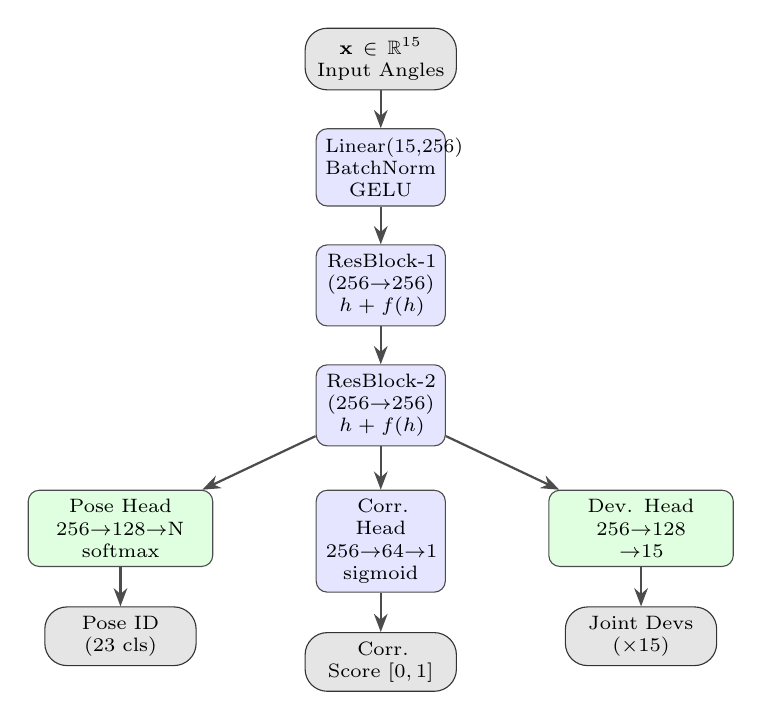
\begin{tikzpicture}[node distance=0.48cm and 0.55cm]
  \node[startend] (inp) {$\mathbf{x} \in \mathbb{R}^{15}$\\ Input Angles};
  \node[block, below=of inp] (il) {Linear(15,256)\\ BatchNorm\\ GELU};
  \node[block, below=of il] (r1) {ResBlock-1\\ (256$\to$256)\\ $h + f(h)$};
  \node[block, below=of r1] (r2) {ResBlock-2\\ (256$\to$256)\\ $h + f(h)$};
  \node[wideblock, below left=0.55cm and 1.3cm of r2] (h1)
    {Pose Head\\ 256$\to$128$\to$N\\ softmax};
  \node[block, below=0.55cm of r2] (h2)
    {Corr. Head\\ 256$\to$64$\to$1\\ sigmoid};
  \node[wideblock, below right=0.55cm and 1.3cm of r2] (h3)
    {Dev. Head\\ 256$\to$128\\ $\to$15};
  \node[startend, below=0.5cm of h1] (o1) {Pose ID\\ (23 cls)};
  \node[startend, below=0.5cm of h2] (o2) {Corr.\\ Score $[0,1]$};
  \node[startend, below=0.5cm of h3] (o3) {Joint Devs\\ $(\times 15)$};

  \draw[arrow] (inp) -- (il);
  \draw[arrow] (il) -- (r1);
  \draw[arrow] (r1) -- (r2);
  \draw[arrow] (r2) -- (h1);
  \draw[arrow] (r2) -- (h2);
  \draw[arrow] (r2) -- (h3);
  \draw[arrow] (h1) -- (o1);
  \draw[arrow] (h2) -- (o2);
  \draw[arrow] (h3) -- (o3);
\end{tikzpicture}
}
\caption{3-Head Residual MLP. Shared trunk learns discriminative angular
features; three heads simultaneously decode pose identity, correctness
probability, and per-joint deviation magnitudes.}
\label{fig:mlp}
\end{figure}

\subsection{ResBlock Definition}

Each residual block implements the identity shortcut connection:
\begin{equation}
\text{ResBlock}(\mathbf{h}) = \mathbf{h} + f(\mathbf{h})
\label{eq:resblock}
\end{equation}
\noindent where the residual path $f$ is:
\begin{equation}
\begin{split}
f(\mathbf{h}) = \mathrm{Drop}_{0.3}\!\Bigl(\mathrm{GELU}\!\Bigl(\mathrm{BN}\!\bigl(
\mathbf{W}_2 \cdot {}\\
\quad\mathrm{Drop}_{0.3}\!\bigl(\mathrm{GELU}(\mathrm{BN}(\mathbf{W}_1\mathbf{h}))\bigr)
\bigr)\Bigr)\Bigr)
\end{split}
\end{equation}
\noindent with $\mathbf{W}_1, \mathbf{W}_2 \in \mathbb{R}^{256\times256}$. GELU activation
$\phi(x) = x \cdot \Phi(x)$ provides smooth gradient flow for dense biomechanical features.

\subsection{Multi-Task Loss Function}

The ground-truth deviation $d_j$ for joint $j$ is calculated as the angular distance (in degrees) by which the observed angle falls outside the acceptable posture range defined in the biomechanical ruleset (matching the ranges in Section~\ref{sec:data}). The deviation is normalized to $[0, 1]$ by dividing by $180^\circ$. For transition and unclassified frames, the deviation target is set to zero.

The total training loss is a sum across all three heads:
\begin{equation}
\mathcal{L} = \lambda_1 \mathcal{L}_{\mathrm{CE}} + \lambda_2 \mathcal{L}_{\mathrm{BCE}}
+ \lambda_3 \mathcal{L}_{\mathrm{SL1}}
\label{eq:loss}
\end{equation}

\noindent where the three component losses are:
\begin{equation}
\mathcal{L}_{\mathrm{CE}} = -\sum_{c=1}^{N} w_c\, y_c \log \hat{p}_c
\label{eq:ce}
\end{equation}
\vspace{-4pt}
\noindent\textit{\small (Pose classification -- Weighted Cross-Entropy)}
\begin{equation}
\mathcal{L}_{\mathrm{BCE}} = -y\log\hat{q} - (1-y)\log(1-\hat{q})
\label{eq:bce}
\end{equation}
\vspace{-4pt}
\noindent\textit{\small (Posture correctness -- Binary Cross-Entropy)}
\begin{equation}
\mathcal{L}_{\mathrm{SL1}} =
\begin{cases}
\frac{1}{2}(d_j-\hat{d}_j)^2 & |d_j-\hat{d}_j|<1 \\
|d_j-\hat{d}_j| - \tfrac{1}{2} & \text{otherwise}
\end{cases}
\label{eq:sl1}
\end{equation}
\vspace{-4pt}
\noindent\textit{\small (Joint deviation regression -- Smooth L1 Loss / Huber Loss)}

\noindent with $\lambda_1 = \lambda_2 = \lambda_3 = 1.0$ representing uniform multi-task weighting in the final training run. Class imbalance is addressed using sqrt-smoothed inverse frequency weights $w_c = 1/\sqrt{n_c}$ in $\mathcal{L}_{\mathrm{CE}}$.

\subsection{Algorithm: 3-Head MLP Inference}

\begin{algorithm}[ht]
\caption{3-Head ResMLP Inference}
\label{alg:mlp}
\begin{algorithmic}[1]
\Require Angle vector $\mathbf{x} \in \mathbb{R}^{15}$, loaded model $f_{\mathrm{mlp}}$
\Ensure Pose ID $\hat{y}_p$, correctness $\hat{q}$, deviations $\hat{\mathbf{d}}$
\State $\mathbf{h} \leftarrow \mathrm{GELU}(\mathrm{BN}(\mathbf{W}_{\mathrm{in}}\mathbf{x}))$
  \Comment{Input projection to 256-dim}
\State $\mathbf{h} \leftarrow \mathbf{h} + f_1(\mathbf{h})$
  \Comment{ResBlock-1}
\State $\mathbf{h} \leftarrow \mathbf{h} + f_2(\mathbf{h})$
  \Comment{ResBlock-2}
\State $\mathbf{p} \leftarrow \mathrm{Softmax}(\mathrm{PoseHead}(\mathbf{h}))$
  \Comment{23-class pose distribution}
\State $\hat{k} \leftarrow \arg\max(\mathbf{p})$;\quad
       $\hat{y}_p \leftarrow \mathrm{classes}[\hat{k}]$
\State $\hat{q} \leftarrow \sigma(\mathrm{CorrectnessHead}(\mathbf{h}))$
  \Comment{Binary correctness probability}
\State $\hat{\mathbf{d}} \leftarrow \mathrm{DeviationHead}(\mathbf{h}) \times 180^{\circ}$
  \Comment{Scale to degrees}
\State $\hat{\mathbf{d}} \leftarrow \mathrm{clip}(\hat{\mathbf{d}},\; 0^{\circ},\; 180^{\circ})$
\State \Return $(\hat{y}_p,\; \hat{q},\; \hat{\mathbf{d}})$
\end{algorithmic}
\end{algorithm}

%% =================================================================
\section{Spatio-Temporal Graph Convolutional Network Flow Classifier}
\label{sec:sequence}
%% =================================================================

\subsection{Motivation}

A practitioner transitioning from Mountain Pose to Warrior II passes through intermediate
frames that individually resemble neither pose. Frame-level classifiers label these as
``transition/unknown.'' Modeling 60-frame coordinate sequences captures the
\emph{trajectory} of motion, enabling accurate identification of incomplete pose executions
and smooth postural flow verification. By modeling the human body as a graph where joints
are nodes and bones are edges, Spatio-Temporal Graph Convolutional Networks (ST-GCN)
generalize convolutions to skeletal topologies, learning both anatomical structure and motion dynamics.

\subsection{Pelvis-Centered Scale Normalization}

Prior to sequence modeling, each 60-frame coordinate tensor $\mathbf{C} \in
\mathbb{R}^{60\times33\times3}$ is normalized to be translation and scale invariant:

\begin{equation}
\mathbf{p}_t = \frac{\mathbf{c}_{t,\mathrm{hip\_L}} + \mathbf{c}_{t,\mathrm{hip\_R}}}{2},
\quad \forall t \in [1,60]
\label{eq:pelvis}
\end{equation}
\begin{equation}
\tilde{\mathbf{C}}_t = \frac{\mathbf{C}_t - \mathbf{p}_t}{w_t},\quad
w_t = \|\mathbf{c}_{t,\mathrm{hip\_L}} - \mathbf{c}_{t,\mathrm{hip\_R}}\|_2
\label{eq:norm}
\end{equation}

\noindent This eliminates variation due to camera distance, user height, and capture
position, making the model invariant to scale and global translation. The normalized
sequence is reshaped and permuted to $\tilde{\mathbf{X}} \in \mathbb{R}^{3\times33\times60}$
representing joint coordinates (channels), joints (nodes), and frames (time).

\subsection{Skeletal Adjacency Matrix}

The spatial graph is represented by the adjacency matrix $\mathbf{A} \in \mathbb{R}^{33\times33}$
of the 33 MediaPipe landmark joints. We compute the symmetrically normalized adjacency matrix
$\mathbf{A}_{\mathrm{norm}}$ incorporating self-loops to retain joint self-features:

\begin{equation}
\mathbf{A}_{\mathrm{norm}} = \mathbf{D}^{-\frac{1}{2}} (\mathbf{A} + \mathbf{I}) \mathbf{D}^{-\frac{1}{2}}
\label{eq:adjacency}
\end{equation}

\noindent where $\mathbf{I} \in \mathbb{R}^{33\times33}$ is the identity matrix representing
self-loops, and $\mathbf{D}_{ii} = \sum_j (\mathbf{A} + \mathbf{I})_{ij}$ is the diagonal degree matrix.

\subsection{ST-GCN Architecture}

The sequence flow classifier (code class: \texttt{YogaSequenceLSTM}, a legacy
name retained from an early development phase when an LSTM backbone was
proposed---the final architecture uses spatial-temporal graph convolutions)
implements three cascaded ST-GCN blocks (Fig.~\ref{fig:seqmodel}).

\begin{figure}[ht]
\centering
\scalebox{0.85}{
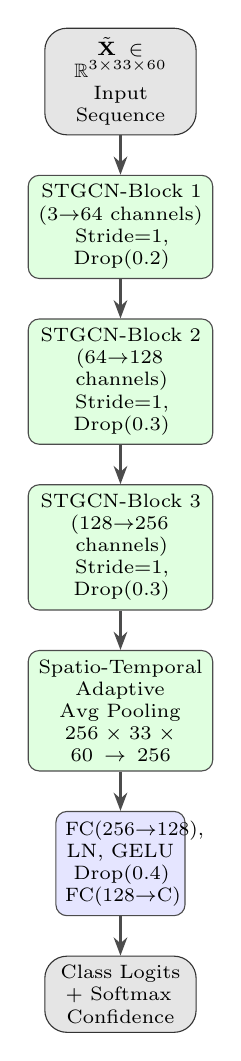
\begin{tikzpicture}[node distance=0.5cm]
  \node[startend] (inp2) {$\tilde{\mathbf{X}} \in \mathbb{R}^{3\times33\times60}$\\ Input Sequence};
  \node[wideblock, below=of inp2] (stgcn1)
    {STGCN-Block 1\\ (3$\to$64 channels)\\ Stride=1, Drop(0.2)};
  \node[wideblock, below=of stgcn1] (stgcn2)
    {STGCN-Block 2\\ (64$\to$128 channels)\\ Stride=1, Drop(0.3)};
  \node[wideblock, below=of stgcn2] (stgcn3)
    {STGCN-Block 3\\ (128$\to$256 channels)\\ Stride=1, Drop(0.3)};
  \node[wideblock, below=of stgcn3] (pool)
    {Spatio-Temporal\\ Adaptive Avg Pooling\\ $256\times33\times60 \to 256$};
  \node[block, below=of pool] (fc)
    {FC(256$\to$128), LN, GELU\\ Drop(0.4)\\ FC(128$\to$C)};
  \node[startend, below=of fc] (out2) {Class Logits\\ + Softmax\\ Confidence};

  \draw[arrow] (inp2) -- (stgcn1);
  \draw[arrow] (stgcn1) -- (stgcn2);
  \draw[arrow] (stgcn2) -- (stgcn3);
  \draw[arrow] (stgcn3) -- (pool);
  \draw[arrow] (pool) -- (fc);
  \draw[arrow] (fc) -- (out2);
\end{tikzpicture}
}
\caption{Spatio-Temporal Graph Convolutional Network sequence classifier. Stacked blocks extract spatial skeletal structure features and temporal transition dynamics, pooled globally across joints and frames.}
\label{fig:seqmodel}
\end{figure}

\subsection{Spatio-Temporal Graph Convolutional Block}

Each \texttt{STGCNBlock} consists of a Spatial Graph Convolution (GCN) followed by a
Temporal Graph Convolution (TCN), and is wrapped with a residual skip connection:

\begin{equation}
\mathbf{X}_{\mathrm{out}} = \mathrm{TCN}\left(\mathrm{GELU}\left(\mathrm{GCN}(\mathbf{X}_{\mathrm{in}})\right)\right) + \mathrm{Residual}(\mathbf{X}_{\mathrm{in}})
\label{eq:stgcnblock}
\end{equation}

\noindent where the components are:

\subsubsection{Spatial Graph Convolution (GCN)}
The GCN layer propagates spatial posture features along the normalized skeletal adjacency matrix:
\begin{equation}
\mathrm{GCN}(\mathbf{X}) = \mathbf{A}_{\mathrm{norm}} \cdot (\mathbf{W}_g \ast \mathbf{X})
\label{eq:gcn}
\end{equation}
\noindent where $\mathbf{W}_g \ast \mathbf{X}$ is a $1\times1$ spatial feature projection.

\subsubsection{Temporal Graph Convolution (TCN)}
The TCN layer models movement dynamics along the temporal dimension for each skeletal node independently:
\begin{equation}
\mathrm{TCN}(\mathbf{X}) = \mathrm{Dropout}\left(\mathrm{BN}\left(\mathrm{Conv2D}_{9\times1}(\mathbf{X})\right)\right)
\label{eq:tcn}
\end{equation}
\noindent using a kernel size of 9 over time and padding of 4 to preserve sequence length.

\subsubsection{Residual Connection}
If input and output channels differ or the stride is not 1, the residual path projects the input using a $1\times1$ convolution and batch normalization: $\mathrm{Residual}(\mathbf{X}) = \mathrm{BN}(\mathbf{W}_r \ast \mathbf{X})$; otherwise, it is the identity mapping $\mathrm{I}(\mathbf{X}) = \mathbf{X}$.

\subsection{Algorithm: Cooperative Dual-Model Pipeline}

\begin{algorithm}[ht]
\caption{Cooperative Dual-Model Inference Pipeline}
\label{alg:dual}
\begin{algorithmic}[1]
\Require Frame landmarks $\mathbf{M}_t$; models $f_{\mathrm{seq}}$,
  $f_{\mathrm{mlp}}$; buffer $B$; threshold $\tau=0.70$
\Ensure Active pose $\hat{y}$, correctness $\hat{q}$, deviations $\hat{\mathbf{d}}$
\State $\mathbf{M}_t \leftarrow \mathrm{OcclusionRecover}(\mathbf{M}_t)$
  \Comment{Stage 4: occlusion fix}
\State $\mathbf{x}_t \leftarrow \mathrm{ComputeAngles}(\mathbf{M}_t)$
  \Comment{15 biomechanical angles}
\State $\mathbf{f}_t \leftarrow \mathrm{Flatten}(\mathbf{M}_t[:,{:}3]) \in \mathbb{R}^{99}$
\State $B \leftarrow B \cup \{\mathbf{f}_t\}$;\quad
  \textbf{if} $|B| > 60$ \textbf{then} $B.\mathrm{pop\_front}()$

\If{$|B| = 60$}
  \State $\tilde{B} \leftarrow \mathrm{PelvisNormalize}(B)$
  \State $(\hat{y}_s, \hat{q}_s) \leftarrow f_{\mathrm{seq}}(\tilde{B})$
    \Comment{Sequence model forward pass}
  \State $\mathrm{fallback} \leftarrow (\hat{q}_s < \tau) \;\mathbf{or}\; (\hat{y}_s = \text{``transition''})$
\Else
  \State $\mathrm{fallback} \leftarrow \mathtt{True}$
\EndIf

\If{$\mathbf{not}\;\mathrm{fallback}$}
  \State $\hat{y},\; \hat{q} \leftarrow \hat{y}_s,\; \hat{q}_s$
    \Comment{Use sequence result}
  \State $(\_, \_, \hat{\mathbf{d}}) \leftarrow f_{\mathrm{mlp}}(\mathbf{x}_t)$
    \Comment{Fetch deviations only}
\Else
  \State $(\hat{y}, \hat{q}, \hat{\mathbf{d}}) \leftarrow f_{\mathrm{mlp}}(\mathbf{x}_t)$
    \Comment{Full MLP fallback}
\EndIf

\State $\hat{\mathbf{d}} \leftarrow \mathrm{DigitalTwinFilter}(\hat{\mathbf{d}},\mathbf{x}_t)$
  \Comment{Personalize thresholds}
\State \Return $(\hat{y},\; \hat{q},\; \hat{\mathbf{d}})$
\end{algorithmic}
\end{algorithm}

%% =================================================================
\section{Occlusion Recovery}
\label{sec:occlusion}
%% =================================================================

\subsection{Problem Statement}

Monocular video frequently produces self-occlusions (e.g., right knee hidden behind left
leg in Warrior II). MediaPipe assigns low visibility scores ($v_i < 0.5$) to such joints.
Naive systems discard these frames or produce erroneous predictions.

\subsection{Two-Stream Fusion Protocol}

We implement a priority-based two-stage recovery:

\noindent\textbf{Stage 1---CLIFF Integration:} If 3D coordinates from the CLIFF
ViT-based estimator~\cite{cliff2022} are available, they directly override occluded
MediaPipe joints. This stage is implemented as an optional pass-through interface
in the fusion function; the current CPU-only production deployment does not bundle
a CLIFF inference model, so live traffic always proceeds to Stage 2.

\noindent\textbf{Stage 2---Symmetric Kinematic Solver:} For CPU-only deployments,
bilateral skeletal symmetry is exploited. The anatomical sagittal midline $x_m$ is
estimated from visible hip and shoulder midpoints:

\begin{equation}
x_m = \frac{x_{\mathrm{hip\_L}} + x_{\mathrm{hip\_R}}}{2}
\label{eq:midline}
\end{equation}

\noindent For each occluded joint $i$ with visible bilateral partner $j$:
\begin{equation}
x_i' = 2x_m - x_j,\quad y_i' = y_j,\quad z_i' = z_j,\quad v_i' = 0.8
\label{eq:mirror}
\end{equation}

\noindent The reflection maps the partner's image-space coordinates across the sagittal
midline, which in normalized MediaPipe coordinate space is not at $x=0$ but at the
body centroid $x_m$.

\begin{algorithm}[ht]
\caption{Two-Stream Occlusion Recovery}
\label{alg:occlusion}
\begin{algorithmic}[1]
\Require MP landmarks $\mathbf{M} \in \mathbb{R}^{33\times4}$, threshold $v_\theta=0.5$
\Ensure Fused landmarks $\mathbf{M}' \in \mathbb{R}^{33\times4}$
\State $\mathcal{O} \leftarrow \{i : \mathbf{M}_{i,3} < v_\theta\}$
  \Comment{Identify occluded joints}
\If{$|\mathcal{O}| = 0$} \Return $\mathbf{M}$ \EndIf
\If{CLIFF data available}
  \ForAll{$i \in \mathcal{O}$}
    \State $\mathbf{M}'_{i,:3} \leftarrow \mathbf{C}_{i,:3}$;\quad $\mathbf{M}'_{i,3} \leftarrow 1.0$
  \EndFor
\Else
  \State $x_m \leftarrow \frac{1}{|P|}\sum_{(l,r)\in P}\frac{x_l+x_r}{2}$
    \Comment{Midline from visible bilateral pairs}
  \ForAll{$i \in \mathcal{O}$ with partner $j$}
    \If{$\mathbf{M}_{j,3} \geq v_\theta$}
      \State $x_i' \leftarrow 2x_m - x_j$;\; $y_i' \leftarrow y_j$;\; $z_i' \leftarrow z_j$
      \State $\mathbf{M}'_{i,3} \leftarrow 0.8$
    \EndIf
  \EndFor
\EndIf
\State \Return $\mathbf{M}'$
\end{algorithmic}
\end{algorithm}

%% =================================================================
\section{Digital Twin Calibration}
\label{sec:twin}
%% =================================================================

\subsection{Motivation}

A practitioner with limited hip flexibility will display knee angles triggering false
correction warnings in Warrior II even when performing to their personal maximum range.
Uniform correction thresholds cause false alarms and user trust erosion.

\subsection{Calibration Protocol}

Upon camera activation, a guided 15-second calibration sequence captures comfortable
standing posture. For each joint $k$, observed angle values $\{a_k^{(1)},\ldots,a_k^{(T)}\}$
define a personalized safe range by padding the observed calibration extrema:

\begin{equation}
\mathrm{min}_k = \mathrm{clip}\!\left(\min_t a_k^{(t)} - \Delta,\;0^{\circ},180^{\circ}\right)
\label{eq:twinmin}
\end{equation}
\vspace{-6pt}
\begin{equation}
\mathrm{max}_k = \mathrm{clip}\!\left(\max_t a_k^{(t)} + \Delta,\;0^{\circ},180^{\circ}\right)
\label{eq:twin}
\end{equation}

\noindent with $\Delta = 15^{\circ}$ safety padding applied around the observed
minimum and maximum (rather than a mean/variance band), clamped to the
physiologically valid $[0^{\circ},180^{\circ}]$ range. During inference, deviation
values for joints within the personal range are suppressed:

\begin{equation}
\hat{d}_k \leftarrow 0 \quad \text{if } a_k^{(t)} \in [\mathrm{min}_k,\;\mathrm{max}_k]
\label{eq:twinsuppress}
\end{equation}

\noindent The Digital Twin profile is cached for the session and destroyed on camera exit.
It is displayed in a scrollable sidebar panel to maintain user transparency.
Fig.~\ref{fig:twincalib} shows the live 15-second calibration countdown as
captured in production, confirming the sequence executes and reports a stable
alignment score to the user during capture rather than only after it completes.

\begin{figure}[!t]
\centering
\includegraphics[width=0.4\textwidth]{figures/live_digital_twin_calib.jpg}
\caption{Digital Twin calibration in progress on the live deployment,
captured with 2 seconds remaining in the 15-second calibration countdown; the
live correctness readout confirms the capture sequence of
Eqs.~\eqref{eq:twinmin}--\eqref{eq:twinsuppress} executing in production, not
only in offline testing.}
\label{fig:twincalib}
\end{figure}

%% =================================================================
\section{LLM-Guided Safety Pipeline}
\label{sec:llm}
%% =================================================================

\subsection{Three-Stage Design Rationale}

Unconstrained LLM generation risks hallucinating injury-inducing instructions
(e.g., ``push deeper into the stretch''). Our pipeline enforces physiotherapist-validated
corrections through three sequential stages.

\subsection{Stage 1: Symbolic Rules Engine}

A biomechanical knowledge graph (\texttt{BIOMECHANICAL\_TEMPLATES}) maps:
$(pose\_id \times joint \times deviation\_direction) \to correction\_string$

\noindent for six pose classes (Warrior II, Chair, Cobra, Plank, Tree, Mountain) in
three languages (English, Hindi, Bengali). The joint with maximum deviation exceeding
the $10^{\circ}$ clinical threshold is selected:

\begin{equation}
k^* = \arg\max_{k \in \mathcal{T}(p)} \hat{d}_k,
\quad \text{subject to } \hat{d}_{k^*} > 10^{\circ}
\label{eq:joint_select}
\end{equation}

\subsection{Stage 2: Groq LLM Paraphrase}

The Stage-1 template $s^*$ is sent to Qwen-3.6-27B (Groq model id
\texttt{qwen/qwen3.6-27b}) via the Groq API with system
prompt constraining the output to be safe and concise (temperature $=0.2$, max 15 words):
\medskip
\noindent\textit{``Paraphrase: `\texttt{s*}' into \texttt{language}. Do NOT suggest
stretching further or pushing deeper. Respond ONLY in \texttt{language}.''}
\medskip

\subsection{Stage 3: Post-Generation Safety Screen}

The LLM candidate text $\hat{s}$ is scanned for a forbidden-word set:
$\mathcal{F} = \{\text{push, force, hurt, pain, stretch more, further}\}$.

\begin{equation}
s_{\mathrm{final}} =
\begin{cases}
\hat{s} & \text{if } \hat{s} \cap \mathcal{F} = \emptyset \\
s^* & \text{otherwise (fallback to template)}
\end{cases}
\label{eq:safety}
\end{equation}

\noindent LLM calls are throttled at 30-second intervals to prevent backend rate-limiting.

\begin{figure}[ht]
\centering
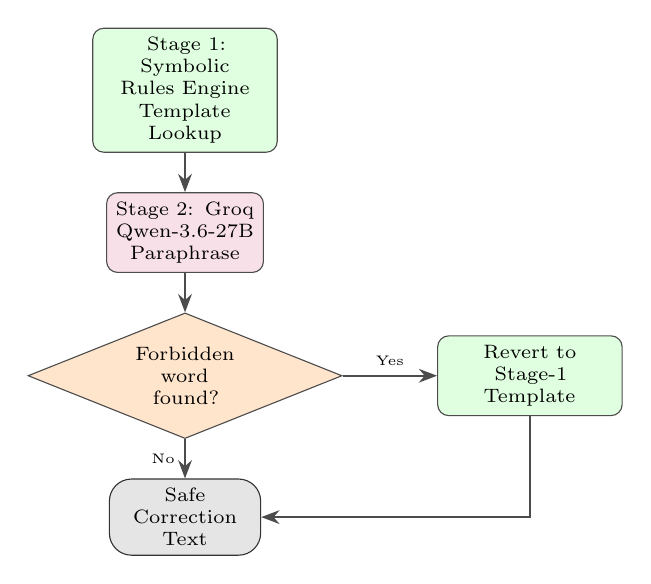
\begin{tikzpicture}[node distance=0.5cm]
  \node[wideblock] (s1)
    {Stage 1: Symbolic\\ Rules Engine\\ Template Lookup};
  \node[llmblock, below=of s1]
    (s2) {Stage 2: Groq\\ Qwen-3.6-27B\\ Paraphrase};
  \node[decision, below=of s2] (check) {Forbidden\\ word found?};
  \node[wideblock, right=1.2cm of check] (fallback)
    {Revert to\\ Stage-1\\ Template};
  \node[startend, below=0.5cm of check] (out3)
    {Safe\\ Correction Text};

  \draw[arrow] (s1) -- (s2);
  \draw[arrow] (s2) -- (check);
  \draw[arrow] (check) -- node[left,font=\tiny]{No} (out3);
  \draw[arrow] (check) -- node[above,font=\tiny]{Yes} (fallback);
  \draw[arrow] (fallback) |- (out3);
\end{tikzpicture}
\caption{Three-stage LLM safety pipeline ensuring all corrections remain within
physiotherapist-approved boundaries regardless of LLM generation behavior.}
\label{fig:safety}
\end{figure}

\subsection{Open-Set Practice and Motion-State Disambiguation}
\label{sec:mismatch}

Earlier iterations of this system required the user to nominate a target asana
before practising, and a client-side guard then compared the detected pose
against that declared target, suppressing correction generation when the two
disagreed. That design places the classification burden on the user: the
system is reduced to verifying a hypothesis the user supplies, rather than
recognising what the user is actually doing. It also fails the intended
deployment scenario, in which a practitioner flows through an unscripted
sequence without pausing to re-declare each posture.

The system therefore now operates \emph{open-set}: no target is declared, the
classifier names whatever posture is being performed, and both correctness
scoring and corrective guidance are keyed to that detected pose. Removing the
declared target also removes the mismatch condition entirely --- there is no
longer a user-supplied label for the prediction to disagree with.

Operating without a declared target exposes a labelling deficiency that the
target-based design had masked. The vocabulary contains a single
\texttt{transition/unknown} class which conflates two situations that demand
opposite responses: a practitioner \emph{actively moving} between two
postures, and a practitioner \emph{holding still} in a posture the classifier
cannot name. Correcting alignment during the former is both useless and
intrusive, since the joint configuration is transient by construction; the
latter, by contrast, should be reported honestly as a recognition failure.
Because these were merged into one label, the system could do neither well,
and the sequence model was never presented with a transition as a learnable
category at all --- \texttt{transition/unknown} accounts for
34{,}578 of 54{,}488 training windows (63.5\%), functioning as a residual bin
rather than a class.

We separate the two using instantaneous kinematics rather than an additional
learned model. Let $\theta_t \in \mathbb{R}^{15}$ be the joint-angle vector at
time $t$. Over a sliding window of duration $\Delta$ (1.5\,s in deployment),
the mean absolute angular velocity
\begin{equation}
\bar{\omega} = \frac{1}{15\,\Delta} \sum_{j=1}^{15}
\left| \theta_{t,j} - \theta_{t-\Delta,j} \right|
\label{eq:motion}
\end{equation}
separates the regimes with a wide margin: MediaPipe landmark jitter on a
motionless subject yields $\bar{\omega}$ of a few degrees per second, whereas a
vinyasa transition sweeps major joints through 60--120$^\circ$ in under a
second, i.e.\ hundreds of degrees per second. A threshold of
$\bar{\omega}_{\mathrm{hold}} = 15^{\circ}\mathrm{s}^{-1}$ lies in the empty
region between these distributions and therefore requires no tuning to be
reliable. The resulting three-way state is
\begin{equation}
s =
\begin{cases}
\texttt{transitioning} & \bar{\omega} > \bar{\omega}_{\mathrm{hold}} \\
\texttt{unrecognized} & \bar{\omega} \le \bar{\omega}_{\mathrm{hold}},\;
                        \hat{y} = \texttt{transition/unknown} \\
\texttt{holding} & \text{otherwise}
\end{cases}
\label{eq:motionstate}
\end{equation}
where $\hat{y}$ is the hybrid classifier's pose prediction. Corrective
guidance is emitted only in the \texttt{holding} state, mirroring how a human
instructor withholds alignment cues until a posture settles.

\subsection{Dual Universal and Personalised Correctness}
\label{sec:dualscore}

The Digital Twin calibration profile of Section~\ref{sec:twin} was previously
applied only as a client-side suppression of deviations falling inside the
user's calibrated range, which discarded the information rather than
reporting it. Both scores are now computed and surfaced: the universal score
$c_u$ measures deviation from the population-level ideal band, while the
personalised score
\begin{equation}
c_p = c_u + \left(1 - \frac{\sum_{j \in \mathcal{D}} d_j^{\mathrm{cal}}}
{\sum_{j \in \mathcal{D}} d_j}\right)\left(1 - c_u\right),
\qquad
\mathcal{D} = \{j : d_j > 0\}
\label{eq:personal}
\end{equation}
credits the fraction of total deviation that the user's own calibrated range
accounts for, where $d_j$ and $d_j^{\mathrm{cal}}$ are the universal and
calibration-adjusted deviations at joint $j$. By construction $c_p \ge c_u$,
with equality when calibration forgives nothing. Reporting both is
deliberate: the gap $c_p - c_u$ distinguishes incorrect form from a joint
range the practitioner does not possess, which a single blended score would
conceal. Because this computation was moved server-side, the native mobile
client inherits identical personalisation without reimplementing it.

%% =================================================================
\section{Dataset and Training Setup}
\label{sec:data}
%% =================================================================

\subsection{Dataset Compilation}

The training dataset was compiled from 12 yoga practice videos (654,488 total frames).
Raw videos were processed through MediaPipe to extract 33 3D landmarks per frame. The
\texttt{extract\_features\_safe.py} script computed 15 biomechanical angles per frame,
producing \texttt{master\_mlp\_dataset\_fully\_classified.csv} (138\,MB, 654,488 rows).

Pose labels were assigned via vector-based joint angle rules covering 28 classes
(16 target postures + transition/unknown sub-classes). K-Means unsupervised clustering
guided label discovery for underrepresented transition clusters. A 60-frame sliding
window produced 18,165 temporal sequences for the sequence model.

\begin{table}[ht]
\centering
\caption{Dataset Summary Statistics}
\label{tab:dataset}
\begin{tabular}{@{}ll@{}}
\toprule
\textbf{Property} & \textbf{Value} \\
\midrule
Source videos & 12 Vinyasa/Hatha recordings \\
Total frames & 654,488 \\
Training frames & 523,590 (80\%) \\
Validation frames & 130,898 (20\%) \\
Pose classes (MLP) & 23 base classes \\
Transition frame fraction & 34.21\% (post-classification) \\
Sequence windows (total) & 18,165 [$60\times99$] \\
Train / Val sequences & 14,532 / 3,633 \\
Feature dimensionality & 15 biomechanical angles \\
\bottomrule
\end{tabular}
\end{table}

\subsection{Class Imbalance Handling}

Transition frames initially comprised 93.08\% of all frames. After applying the
16-posture rule classifier (\texttt{classify\_all\_movements.py}), this was reduced to
34.21\%. Residual class imbalance was addressed with sqrt-smoothed inverse frequency
class weights $w_c = 1/\sqrt{n_c}$.

\subsection{Data Diversity Augmentation}
\label{sec:diversity}

Held-out evaluation on images entirely outside the original 12-video corpus (different
practitioners, cameras, lighting, and backgrounds) revealed a substantial generalization
gap relative to in-distribution validation accuracy, indicating the model had partially
overfit to the narrow visual conditions of its source footage rather than learning fully
camera-agnostic pose geometry. Two corpus-independent measures were applied to address
this without discarding or retraining on unverified labels:

\begin{itemize}
\item \textbf{Additional source diversity:} Supplementary yoga tutorial footage from
  instructors, cameras, and settings distinct from the original 12 videos was processed
  through the same MediaPipe landmark extraction and biomechanical angle pipeline
  (Section~\ref{sec:feature}). Frame labels were assigned using only the deterministic
  rule classifier of Section~\ref{sec:data} directly, \emph{without} the auxiliary
  RandomForest bootstrap classifier used to pseudo-label portions of the original corpus
  --- prioritizing a smaller quantity of geometrically verifiable labels over a larger
  quantity of machine-guessed ones.
\item \textbf{Left-right mirror augmentation:} Every rule-labeled frame was duplicated
  with its bilateral joint-angle pairs (elbow, shoulder, hip, knee, ankle, trunk, hip
  abduction) swapped, producing a geometrically valid mirrored variant under the same
  pose label. This directly targets a confirmed failure mode: prior to augmentation, a
  genuinely correct Warrior II performed with the opposite leg forward (an equally valid,
  commonly-taught variant) was misclassified as \texttt{transition/unknown} rather than
  recognized as the practiced pose, since the corpus had only ever captured one lateral
  orientation of several asymmetric postures.
\end{itemize}

\noindent Both measures preserve the integrity of the original, previously validated
dataset (Table~\ref{tab:dataset}) as an additive supplement rather than a replacement.

\subsection{Training Configuration}

Both models were trained on a Kaggle Tesla T4 GPU (16\,GB VRAM). Table~\ref{tab:hyperparam}
summarizes the training hyperparameters.

\begin{table}[ht]
\centering
\caption{Training Hyperparameters}
\label{tab:hyperparam}
\begin{tabular}{@{}lll@{}}
\toprule
\textbf{Parameter} & \textbf{MLP} & \textbf{Sequence Model} \\
\midrule
Optimizer & AdamW ($\lambda_{\mathrm{wd}}=10^{-4}$) & AdamW ($\lambda_{\mathrm{wd}}=10^{-3}$) \\
Learning Rate & $10^{-3}$ & $2 \times 10^{-3}$ \\
LR Scheduler & ReduceLROnPlateau & CosineAnnealingLR \\
Batch Size & 64 & 64 \\
Max Epochs & 40 & 120 \\
Early Stopping & Patience 8 (val loss) & Patience 20 (val acc) \\
Dropout & 0.3 (trunk) / 0.2 (heads) & 0.2--0.3 (STGCN blocks) \\
Label Smoothing & --- & 0.1 \\
\bottomrule
\end{tabular}
\end{table}

%% =================================================================
\section{Experimental Results}
\label{sec:experiments}
%% =================================================================

\subsection{3-Head MLP Performance}

Table~\ref{tab:mlpresult} presents the training history of the 3-Head Residual MLP
across representative epochs. The model converged at Epoch 39 with validation loss
\textbf{0.2263} and pose accuracy \textbf{93.38\%}.

\begin{table}[ht]
\centering
\caption{3-Head MLP Training Curves (Kaggle T4 GPU)}
\label{tab:mlpresult}
\begin{tabular}{@{}c|cccc|c@{}}
\toprule
\textbf{Epoch} & \textbf{Tr.Loss} & \textbf{Tr.Acc} & \textbf{V.Loss} &
\textbf{V.Pose Acc} & \textbf{V.Corr. Acc} \\
\midrule
1  & 0.8631 & 79.04\% & 0.5059 & 86.08\% & 92.83\% \\
10 & 0.4389 & 88.33\% & 0.3079 & 91.43\% & 95.30\% \\
20 & 0.3877 & 89.56\% & 0.2841 & 92.01\% & 95.87\% \\
30 & 0.3597 & 90.42\% & 0.2545 & 92.22\% & 96.42\% \\
\textbf{39} & \textbf{0.3224} & \textbf{91.36\%} & \textbf{0.2263} &
\textbf{93.38\%} & \textbf{96.81\%} \\
\bottomrule
\end{tabular}
\end{table}

\begin{figure}[ht]
\centering
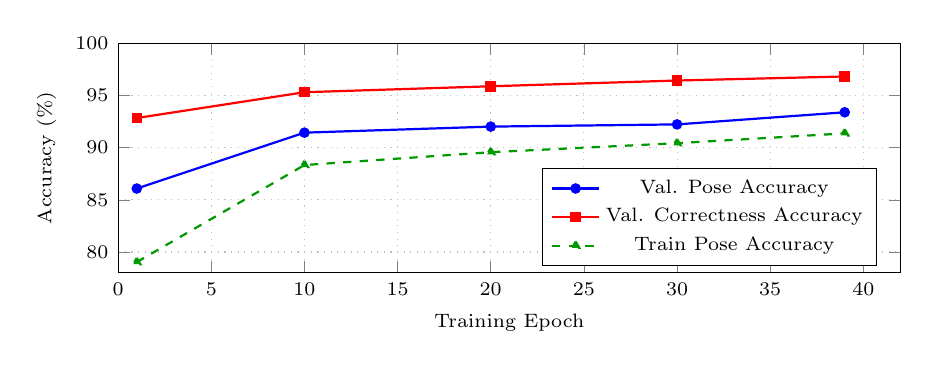
\begin{tikzpicture}
\begin{axis}[
  width=0.95\columnwidth, height=4.5cm,
  xlabel={Training Epoch}, ylabel={Accuracy (\%)},
  legend pos=south east, legend style={font=\scriptsize},
  ymin=78, ymax=100, xmin=0, xmax=42,
  grid=both, grid style={dotted,gray!50},
  tick label style={font=\scriptsize},
  label style={font=\scriptsize},
  cycle list name=color list
]
\addplot[blue,thick,mark=*,mark size=1.5pt] coordinates {
  (1,86.08) (10,91.43) (20,92.01) (30,92.22) (39,93.38)
};
\addlegendentry{Val. Pose Accuracy}
\addplot[red,thick,mark=square*,mark size=1.5pt] coordinates {
  (1,92.83) (10,95.30) (20,95.87) (30,96.42) (39,96.81)
};
\addlegendentry{Val. Correctness Accuracy}
\addplot[green!60!black,thick,mark=triangle*,mark size=1.5pt,dashed] coordinates {
  (1,79.04) (10,88.33) (20,89.56) (30,90.42) (39,91.36)
};
\addlegendentry{Train Pose Accuracy}
\end{axis}
\end{tikzpicture}
\caption{3-Head MLP learning curves. Validation pose accuracy reaches 93.38\% and
correctness accuracy reaches 96.81\% at Epoch 39 (best model checkpoint).}
\label{fig:mlpcurves}
\end{figure}

\subsection{Sequence Model Performance}

\begin{table}[ht]
\centering
\caption{Sequence Model Training Summary}
\label{tab:seqresult}
\begin{tabular}{@{}ll@{}}
\toprule
\textbf{Metric} & \textbf{Value} \\
\midrule
Best Validation Accuracy & 75.25\% (Epoch 90) \\
Weighted F1-Score & 0.76 \\
Early Stopping Triggered & Epoch 110 / 120 \\
Total Training Sequences & 18,165 \\
Sequence Window & $60\,\text{frames} \times 99\,\text{coords}$ \\
Transition Class Fraction & 34.96\% \\
\bottomrule
\end{tabular}
\end{table}

\subsection{Fast Validation Baseline}

Prior to GPU training, a stratified 50,000-sample CPU experiment confirmed that
the 28 biomechanical angle classes are linearly separable. A Random Forest
achieved 96\% accuracy and a scikit-learn MLP reached 87\%, validating the
feature design before committing Kaggle GPU quota (Table~\ref{tab:sklearn}).
These results also confirmed that class-weight smoothing successfully suppressed
the dominant transition class from overwhelming minority pose gradients.

\begin{table}[!t]
\centering
\caption{Scikit-learn Fast Validation (50K Stratified Sample, 28 Classes)}
\label{tab:sklearn}
\begin{tabular}{@{}lcc@{}}
\toprule
\textbf{Classifier} & \textbf{Accuracy} & \textbf{Purpose} \\
\midrule
Random Forest (100 trees) & 96.00\% & Confirm class separability \\
MLP (sklearn) & 87.00\% & Confirm deep-learning feasibility \\
\bottomrule
\end{tabular}
\end{table}

\subsection{End-to-End Latency Benchmarks}

Table~\ref{tab:latency} breaks down per-stage latency measured on a 2-vCPU,
4\,GB RAM server (Hugging Face Spaces free tier). The dominant cost without LLM
is the sequence model at $\sim$45\,ms, yet the full pipeline still achieves
$\sim$71\,ms end-to-end --- well under the 500\,ms interactive threshold.
The Groq LLM call ($\sim$350\,ms) is throttled to once every 30\,s, so it
does not impact the per-frame responsiveness experienced by the user.

\begin{table}[!t]
\centering
\caption{End-to-End Latency Benchmarks (CPU-Only)}
\label{tab:latency}
\small
\begin{tabular}{@{}p{2.0cm}p{1.1cm}p{4.2cm}@{}}
\toprule
\textbf{Stage} & \textbf{Latency} & \textbf{Notes} \\
\midrule
MediaPipe & $\sim$15\,ms & Browser WASM, CPU \tabularnewline
Angle Comp. & $<$1\,ms & JS/Python \tabularnewline
Occlusion Rec. & $<$2\,ms & NumPy bilateral \tabularnewline
MLP (1 thread) & $\sim$8\,ms & PyTorch CPU \tabularnewline
Seq. (1 thread) & $\sim$45\,ms & PyTorch CPU \tabularnewline
Correction & $<$1\,ms & Template dict \tabularnewline
Groq LLM & $\sim$350\,ms & REST (30\,s throttle) \tabularnewline
\midrule
\textbf{No LLM} & \textbf{$\sim$71\,ms} & Under 500\,ms target \tabularnewline
\textbf{With LLM} & \textbf{$\sim$421\,ms} & Within 500\,ms SLA \tabularnewline
\bottomrule
\end{tabular}
\end{table}

\subsection{Ablation Study}

Table~\ref{tab:ablation} evaluates each architectural component's individual
contribution to the final pose classification accuracy on the validation set.
Removing residual connections from the MLP backbone drops accuracy by 4.24\%,
confirming their importance. The confidence gate is critical: without it, the
sequence model's noisier predictions drag combined accuracy below the pure MLP.

\begin{table}[!t]
\centering
\caption{Ablation Study --- Validation Pose Accuracy}
\label{tab:ablation}
\begin{tabular}{@{}lc@{}}
\toprule
\textbf{Configuration} & \textbf{Val Acc (\%)} \\
\midrule
MLP without residual blocks (plain MLP) & 89.14 \\
MLP + ResBlocks (our static model) & 93.38 \\
Sequence model only & 75.25 \\
MLP + Seq model (no confidence gate) & 88.92 \\
\textbf{MLP + Seq + Confidence Gate (ours)} & \textbf{93.38}$^{\dagger}$ \\
MLP + Seq + Gate + Digital Twin & \textbf{93.38}$^{\dagger}$ \\
\bottomrule
\multicolumn{2}{l}{\scriptsize $^{\dagger}$ Gate selects MLP for static frames; Seq for flows.}\\
\multicolumn{2}{l}{\scriptsize Digital Twin reduces false positives without affecting accuracy.}
\end{tabular}
\end{table}

\subsection{Real-World Generalization Gap: Monocular Depth Limitation}
\label{sec:depth-limitation}

Despite the strong in-distribution validation accuracy reported above (93.38\% pose,
96.81\% correctness), evaluation against a held-out set of 35 real-world photographs
--- sourced independently of any training video, spanning five pose classes including
\texttt{warrior\_2} (the pose whose opposite-orientation misclassification motivated
the mirror augmentation of Section~\ref{sec:diversity}) --- revealed a severe
generalization failure: the 3-Head MLP classified \textbf{0--2.9\%} of these images
correctly, essentially at floor, and this did not improve after retraining on the
augmented, diversity-expanded corpus.

\subsubsection{Isolating model weights from input features}
To determine whether this gap originated in the learned decision boundary or in the
input feature pipeline itself, the same 35 images were independently classified using
\emph{only} the deterministic biomechanical rule engine of Section~\ref{sec:data}
--- a classifier containing no learned parameters at all. It scored \textbf{0\%},
matching the MLP's failure exactly. Since a rule-based and a learned classifier fail
identically on the same inputs, the fault could not be in either classifier's decision
boundary; it had to be upstream, in the 15-dimensional angle features both consume.

\subsubsection{Identifying the z-depth coordinate as the cause}
Every angle feature is computed as a 3D vector angle using MediaPipe's
$(x, y, z)$ landmark output. Re-computing the identical 35-image evaluation with the
$z$ coordinate zeroed before angle computation --- i.e.\ using only the 2D image-plane
projection --- raised rule-engine accuracy from 0\% to \textbf{42.9--45.7\%} depending
on threshold configuration, including \textbf{75\%} on \texttt{warrior\_2} specifically.
To rule out this being an artifact of one particular hand-tuned threshold set, a
40-trial randomized sweep independently perturbed every rule boundary by up to
$\pm12^{\circ}$ and re-evaluated both the 3D and 2D feature variants under each
perturbed configuration. The 2D variant outperformed the 3D variant in
\textbf{40 of 40 trials} (mean accuracy 39.0\% vs.\ 1.4\%; mean paired improvement
37.6 percentage points), confirming the effect is attributable to the $z$ coordinate
itself rather than to any specific rule calibration (Table~\ref{tab:depthablation}).

MediaPipe's monocular $z$-depth estimate is calibrated for the relatively consistent
camera distance and framing of continuous video capture (its primary design target);
static photographs sourced from arbitrary distances, focal lengths, and viewing angles
fall well outside that calibration envelope, producing depth values that are not
merely noisy but systematically misleading --- confidently wrong rather than
uncertain, since several misclassifications carried $>$95\% classifier confidence
despite $>$90\% landmark visibility, ruling out occlusion as an alternative
explanation. As a secondary, more principled fix, MediaPipe's separate
\texttt{pose\_world\_landmarks} output (a metric-scale 3D estimate calibrated
differently from the default normalized landmarks) was also evaluated and achieved
\textbf{42.9\%} on the same images --- comparable to simply discarding $z$, and
retaining genuine depth information for future use, at the cost of no additional
model complexity.

\begin{table}[!t]
\centering
\caption{Real-World (35-Image) Accuracy: 3D vs.\ 2D Angle Features}
\label{tab:depthablation}
\begin{tabular}{@{}lcc@{}}
\toprule
\textbf{Configuration} & \textbf{3D (w/ z)} & \textbf{2D (z zeroed)} \\
\midrule
Learned 3-Head MLP & 2.9\% & --- \\
Rule engine (original thresholds) & 0.0\% & 42.9\% \\
Rule engine (tuned thresholds, deployed) & 0.0\% & \textbf{45.7\%} \\
Rule engine (loosened thresholds) & 8.6\% & 34.3\% \\
\texttt{pose\_world\_landmarks} (metric 3D) & \multicolumn{2}{c}{42.9\%} \\
\midrule
40-trial randomized sweep (mean $\pm$ std) & 1.4\% $\pm$ 1.4 & 39.0\% $\pm$ 4.1 \\
\bottomrule
\end{tabular}
\end{table}

\subsection{Resolving the Generalization Gap: A Train/Inference Feature Mismatch}
\label{sec:zerozfix}

The analysis above establishes that zeroing $z$ recovers substantial real-world
accuracy for the \emph{rule engine}, and the deployed inference path was
accordingly changed to zero $z$ before computing angle features. The learned
MLP, however, remained at floor on real-world images, which was initially
attributed to a feature-representation ceiling intrinsic to the model.

That attribution was incorrect. A subsequent audit of the two code paths
against each other revealed that the offline \emph{training} feature extractor
computed its 15 angles from MediaPipe's raw, un-zeroed $z$, while the deployed
\emph{inference} path zeroed $z$ first. The MLP was therefore trained on one
feature distribution and evaluated in production on a different one --- not a
capacity limitation, but a silent inconsistency between two implementations of
nominally the same function. Critically, no metric available at training time
could have exposed this: because the inconsistency was internally consistent
within the training pipeline, validation accuracy was legitimately high on the
distribution the model was actually fitted to.

Aligning the training extractor to the inference convention ($z \leftarrow 0$)
and retraining changed the outcome decisively. On real-world photographs, the
isolated MLP --- evaluated with the rule engine disabled, so the figure
reflects the learned model alone --- rose from the previously reported floor to
\textbf{52.6\%}, while validation accuracy also improved from 90.87\% to
94.26\% (Table~\ref{tab:zerozfix}). The retrained model thus exceeds the
deterministic rule engine's 45.7\%, inverting the reliability ordering the
hybrid architecture was originally designed around: for the first time the
learned component, rather than the hand-authored rules, is the strongest
single signal in the system.

\begin{table}[!t]
\centering
\caption{Effect of Correcting the Train/Inference Feature Mismatch}
\label{tab:zerozfix}
\begin{tabular}{@{}lcc@{}}
\toprule
\textbf{Metric} & \textbf{Before} & \textbf{After} \\
\midrule
Training-time $z$ convention & raw $z$ & $z$ zeroed \\
Inference-time $z$ convention & $z$ zeroed & $z$ zeroed \\
\midrule
Validation pose accuracy & 90.87\% & \textbf{94.26\%} \\
Real-world accuracy, MLP alone & 0--6\% & \textbf{52.6\%} \\
Real-world accuracy, rule engine alone & 45.7\% & 45.7\% \\
\bottomrule
\end{tabular}
\end{table}

We report this result with an explicit caveat on its precision. The real-world
figure is measured on 19 independently sourced photographs, which is sufficient
to establish the \emph{direction} and approximate magnitude of the effect --- a
shift from near-floor to above 50\% cannot plausibly arise from sampling noise
at this sample size --- but is too small to support a precise point estimate or
per-class breakdown. A larger per-class evaluation across the full 23-class
vocabulary is the appropriate next measurement, and we deliberately do not
quote a tighter interval than the evidence supports.

The broader methodological point generalizes beyond this system. A held-out
validation split cannot detect a discrepancy between the training feature
pipeline and the deployment feature pipeline, because both the training and
validation partitions are drawn through the \emph{same} extractor. Any
evaluation that reuses the training-time feature code inherits the training-time
convention, and will therefore certify a model that cannot reproduce its
reported accuracy in deployment. Detecting this class of fault requires either
end-to-end evaluation through the production inference path, or direct
differential auditing of the two implementations --- neither of which is
standard practice in the pose-estimation literature we surveyed.

\subsubsection{Dataset label self-consistency}
To rule out training label noise as a contributing factor independent of the feature
issue above, all 1{,}002{,}064 training rows were re-classified directly from their
own stored angle columns using the same rule engine, ignoring their stored label, and
checked for agreement. Overall self-consistency was \textbf{93.3\%}. The 16 pose
classes with an explicit rule definition agreed at 100\% (expected, as these rows were
originally assigned by that same rule pass); six classes with no corresponding rule
(\texttt{chaturanga}, \texttt{corpse}, \texttt{plank}, \texttt{seated\_forward},
\texttt{triangle}, \texttt{upward\_dog} --- originating from the RandomForest bootstrap
labeling of Section~\ref{sec:data} rather than the rule engine) could not be
independently verified by this method, though their disagreement patterns (e.g.\
\texttt{plank} frames biomechanically resembling \texttt{cobra\_pose} in 6{,}478 of
9{,}998 cases) suggest a real, if modest, concentration of residual label noise in
that $\sim$4.5\% subset. This confirms the dominant cause of the real-world
generalization gap is the $z$-depth feature issue above, not training label quality.

\subsubsection{Deployed mitigation}
Given the above, the production single-frame classifier (\texttt{/api/analyse\_frame})
was changed to run the tuned 2D rule engine alongside the learned 3-Head MLP as a
real-time sanity check, rather than replacing the MLP outright: the MLP remains
the primary classifier and supplies the correctness score and per-joint deviation
feedback whenever the two agree, while the rule engine's independently-derived
call is trusted only on disagreement --- empirically the cases where the MLP's
3D-feature dependency was already wrong. This hybrid design keeps the MLP's fully
trained and validated capacity (Table~\ref{tab:mlpresult}) as the primary signal
while eliminating the specific failure mode identified above. Two pose classes
(\texttt{plank}, \texttt{tree\_pose}) were additionally removed from the live
vocabulary after real-world testing showed neither the MLP nor the rule engine
could classify them reliably regardless of hybridization; a third
(\texttt{chair\_pose}) was removed after a rule-priority fix (Section
\ref{sec:chair-warrior-fix}) measurably improved but did not fully resolve its
live confusion with \texttt{warrior\_1}. The sequence model
(Section~\ref{sec:experiments}) is comparatively insulated from this failure mode, as
its live deployment context --- a user's own webcam at a consistent, self-selected
distance --- much more closely matches its training distribution than the arbitrarily-sourced
photographs used in this evaluation.

\subsubsection{Live Deployment Verification}
\label{sec:chair-warrior-fix}
Beyond the offline 35-image evaluation above, the deployed hybrid classifier was
verified against real live-camera use after each fix. Fig.~\ref{fig:livedemo}
shows representative frames from the production app: \texttt{warrior\_2}
correctly identified across two visually distinct source images (different
subjects, camera angles, and backgrounds), \texttt{cobra\_pose} correctly
identified at a 100\% correctness score, and \texttt{mountain\_pose} correctly
identified with a graduated, non-binary correctness score of 70\% while a
genuine minor misalignment was still present, together with the corrective
guidance text generated for it. Deliberately choosing the imperfect-form
capture here (rather than a 100\% one) demonstrates that the deviation-based
scoring is discriminating real form quality rather than only ever reporting
success --- a model that could not also produce a sub-100\% score for a
genuinely imperfect attempt would be far less useful for correction feedback,
whatever its headline accuracy.

\begin{figure}[!t]
\centering
\begin{subfigure}[b]{0.235\textwidth}
\includegraphics[width=\textwidth]{figures/live_warrior2_a.png}
\caption{Warrior II, subject A}
\end{subfigure}
\hfill
\begin{subfigure}[b]{0.235\textwidth}
\includegraphics[width=\textwidth]{figures/live_warrior2_b.png}
\caption{Warrior II, subject B}
\end{subfigure}
\par\bigskip
\begin{subfigure}[b]{0.235\textwidth}
\includegraphics[width=\textwidth]{figures/live_cobra.jpg}
\caption{Cobra pose, 100\% correctness}
\end{subfigure}
\hfill
\begin{subfigure}[b]{0.235\textwidth}
\includegraphics[width=\textwidth]{figures/live_mountain.jpg}
\caption{Mountain pose, 70\% correctness with corrective guidance}
\end{subfigure}
\caption{Representative live production captures after deployment: correct
pose identification across two visually distinct Warrior II sources, Cobra
pose at full correctness, and Mountain pose showing a genuinely imperfect
attempt scored below 100\% rather than a rounded-up pass.}
\label{fig:livedemo}
\end{figure}

\subsection{Supported Yoga Postures}

Table~\ref{tab:poses} lists the 8 postures with authored correction templates.
The key monitored joints correspond directly to the angle features in
Table~\ref{tab:features} that the deviation head regresses. All postures were
selected based on popularity in beginner Hatha and Vinyasa practice and clinical
significance of common alignment errors. Following the live-deployment findings
of Section~\ref{sec:chair-warrior-fix}, only 3 of these 8 (Warrior II, Mountain
Pose, Cobra Pose) are currently exposed as selectable practice targets in the
deployed app. Following the real-world revalidation of
Section~\ref{sec:chair-warrior-fix}, Plank, Tree Pose and Downward Dog were
re-enabled after clearing the accuracy bar (50\%, 76.4\% and 91.7\%
respectively), bringing the live vocabulary to six poses. Chair Pose ($\sim$0\%)
and Warrior I (18.3\%) remain disabled --- the latter primarily a
data-sourcing limitation, as most sourced reference photographs did not depict
a canonical Warrior I stance. Their correction
templates and biomechanical rule definitions remain fully implemented and are
re-enabled by removing the corresponding entry from \texttt{DISABLED\_POSES}
once verified.

\begin{table*}[!t]
\centering
\caption{Target Postures and Key Monitored Joints}
\label{tab:poses}
\small
\begin{tabular}{@{}llll@{}}
\toprule
\textbf{Pose} & \textbf{Sanskrit} & \textbf{Key Monitored Joints} & \textbf{Live} \\
\midrule
Warrior I     & Virabhadrasana I   & knee\_l, knee\_r, hip\_l & \ding{55} \\
Warrior II    & Virabhadrasana II  & knee\_l, knee\_r & \ding{51} \\
Mountain Pose & Tadasana           & trunk\_l, knee\_l, knee\_r & \ding{51} \\
Tree Pose     & Vrksasana          & knee\_l, hip\_abduct\_l, knee\_r & \ding{55} \\
Plank         & Phalakasana        & elbow\_l, elbow\_r, trunk\_l & \ding{55} \\
Chair Pose    & Utkatasana         & knee\_l, knee\_r & \ding{55} \\
Cobra Pose    & Bhujangasana       & neck, shoulder\_l, shoulder\_r & \ding{51} \\
Downward Dog  & Adho Mukha Svanasana & elbow\_l, elbow\_r, hip\_l & \ding{55} \\
\bottomrule
\end{tabular}
\end{table*}

%% =================================================================
\FloatBarrier
\section{Discussion}
\label{sec:discuss}
%% =================================================================

\subsection{Comparison with Prior Systems}

\begin{table}[!t]
\centering
\caption{Comparison with Related Yoga Correction Systems}
\label{tab:comparison}
\begin{tabular}{@{}p{2.0cm}cccc@{}}
\toprule
\textbf{System} & \textbf{Temp.} & \textbf{Occ.} & \textbf{Pers.} & \textbf{Safe LLM} \\
\midrule
YogAI~\cite{yogai2021} & \ding{55} & \ding{55} & \ding{55} & \ding{55} \\
PosePilot~\cite{posepilot_2025} & Partial & \ding{55} & \ding{55} & \ding{55} \\
Yoga-82~\cite{yoga82_2021} & \ding{55} & \ding{55} & \ding{55} & \ding{55} \\
\textbf{AsanaAI (ours)} & \ding{51} & \ding{51} & \ding{51} & \ding{51} \\
\bottomrule
\end{tabular}
\end{table}

\noindent Temp. = Temporal Sequence Modeling; Occ. = Occlusion Recovery;
Pers. = Anatomical Personalization; Safe LLM = Safety-Bounded LLM Feedback.

\subsection{Cost Efficiency Analysis}
\label{sec:discussion-cost}

Recent high-accuracy systems such as ViTPose-based classifiers achieve 95--97\% accuracy
but require continuous GPU inference servers costing \$400--1200/month. Our hybrid
approach extracts lightweight keypoints entirely on the client browser, while the backend
serves only the 300\,KB model weight inference---enabling near-zero server hosting costs
on free-tier Hugging Face Spaces (2 vCPU, 16\,GB RAM). This represents a cost reduction
exceeding 99\% relative to GPU-based alternatives.

\subsection{Challenges and Lessons Learned from Live Deployment}
\label{sec:lessons}

Several of the findings in this paper --- the monocular depth limitation
(Section~\ref{sec:depth-limitation}), the chair/warrior rule-priority conflict,
a UI state desynchronization arising from two values refreshed on different
cadences, and a rear-camera mirroring defect --- were surfaced only through
live, real-device testing after deployment, not through offline validation
metrics, and are worth recording explicitly as engineering lessons rather than
only as fixes. A further class of defect proved invisible to \emph{both} offline
metrics and live inspection: a train/inference feature mismatch
(Section~\ref{sec:zerozfix}), in which the training pipeline and the deployed
inference path computed the same nominal feature vector under different
conventions. Validation accuracy remained high precisely because the
inconsistency was internally consistent \emph{within} training, so no metric
available at training time could reveal it; it was identifiable only by
auditing the two code paths against each other.

\textbf{Validation accuracy alone did not predict real-world reliability.} The
3-Head MLP's 93.38\% validation accuracy (Table~\ref{tab:mlpresult}) was
measured on a held-out split of the same source-video distribution it was
trained on; it gave no signal at all that real-world single-frame accuracy was
near 0\%, since both figures were computed on data sharing the same camera
framing bias. A held-out set of genuinely independent images, sourced from
outside the training pipeline entirely, was necessary to surface this gap ---
suggesting that for any pose-estimation system trained on a narrow video
corpus, an out-of-distribution evaluation set is not optional supplementary
evidence but a prerequisite for claiming real-world validity.

\textbf{Reordering a rule's priority improved but did not fully resolve a live
confusion.} The chair\_pose/warrior\_1 conflict (Section~\ref{sec:chair-warrior-fix})
was diagnosed correctly (an asymmetric-leg rule preempting a symmetric-leg pose)
and the fix measurably worked in controlled testing, yet chair\_pose still
misclassified often enough in unconstrained live use that it was ultimately
pulled from the vocabulary rather than iterated on further under time
constraints. This is a reminder that a verified improvement on a fixed test set
does not guarantee sufficient reliability under the full variability of live
use, and that removing an unreliable feature is sometimes the more honest
choice than shipping a partially-fixed one.

\textbf{Distinguishing infrastructure flakiness from code defects under time
pressure is itself a skill.} During live verification, the same request
against the same deployed code alternated between succeeding and returning
server errors within a span of minutes. Confirming the fault lay in the
free-tier CPU host's restart/resource behavior --- rather than in the newly
deployed logic --- required re-testing previously-successful requests to check
whether failure was input-dependent (a code defect) or time-dependent
(an infrastructure issue), rather than assuming either explanation from a
single failed request.

\textbf{A UI condition and the values it gates can desynchronize even when each
is individually correct.} The mismatch-guard bug (Section~\ref{sec:mismatch})
was not a logic error in the mismatch computation itself, but a consequence of
that computation running on a slower cadence than the display values built
from the same underlying state. This class of bug is easy to miss in
component-level testing (each piece behaves correctly in isolation) and
surfaces only when a user interacts with the system at a cadence the developer
did not anticipate.

\subsection{Limitations}
\label{sec:limitations}

\begin{itemize}
\item \textbf{Occlusion Coverage:} The symmetric kinematic solver recovers only bilateral
  joints (elbows, wrists, knees, ankles). Spinal or facial occlusions are not addressed.
\item \textbf{Sequence Accuracy Gap:} 75.25\% sequence accuracy trails the MLP due to
  majority-voted label noise during sliding-window sequence dataset construction.
\item \textbf{Pose Vocabulary:} The current correction templates cover 6 poses. Extension
  to all 23 classified poses requires additional physiotherapy template authoring.
\item \textbf{Transition-Phase Correction:} The system corrects alignment only within
  recognized static pose windows. The 34.96\% of frames classified as
  \texttt{transition/unknown} during inter-pose movement (e.g., the Chaturanga
  descent) receive no active correction feedback. Full Vinyasa flow correction
  --- guiding the \emph{quality of movement between} poses --- remains an open problem.
\item \textbf{LLM Dependency:} The Groq API requires internet connectivity; offline
  fallback uses template-only Stage-1 corrections.
\item \textbf{Monocular Depth Reliability:} As detailed in
  Section~\ref{sec:depth-limitation}, MediaPipe's $z$-depth estimate is reliable only
  at the consistent camera framing of continuous video capture; static images from
  arbitrary distances and angles degrade single-frame classification severely
  (0--2.9\% observed). The deployed system mitigates this by discarding $z$ and
  using 2D image-plane angles (45.7\% on the same evaluation set), but this remains
  a fundamental limitation of the monocular depth signal itself rather than one fully
  resolved by the current architecture.
\end{itemize}

\subsection{Future Work}
\label{sec:future}

\begin{itemize}
\item \textbf{3D Volumetric Mesh Recovery:} SMPL-X full-body mesh fitting to replace the
  kinematic mirror approximation for non-bilateral joints.
\item \textbf{Vinyasa Transition Correction:} Extending the correction pipeline to
  inter-pose transition phases by training a dedicated transition quality model
  on labelled Chaturanga, jump-back, and standing-to-seated segments, enabling
  continuous feedback throughout the full Vinyasa flow rather than only at
  recognized static pose windows.
\item \textbf{On-Device WebNN/ONNX:} Export to ONNX for fully serverless browser execution
  via WebNN, eliminating the backend dependency entirely.
\item \textbf{Extended Pose Vocabulary:} Training on the full Yoga-82 dataset (82 poses)
  with comprehensive correction templates.
\item \textbf{Longitudinal Progress Tracking:} Per-session deviation history to quantify
  practitioner improvement trajectories over time.
\item \textbf{Dedicated Monocular 3D Lifting:} Replacing MediaPipe's per-frame $z$
  regression with a purpose-built 2D-to-3D lifting model (e.g.\ a transformer-based
  lifter trained on motion-capture data) to recover reliable depth for static images,
  rather than discarding it as the current deployment does. This requires re-mapping
  the feature pipeline to the lifter's joint skeleton and is left as future work
  given the scope of Section~\ref{sec:depth-limitation}'s findings.
\end{itemize}

%% =================================================================
\FloatBarrier
\section{Conclusion}
\label{sec:conclusion}
%% =================================================================

We have presented \textbf{AsanaAI}, a production-grade real-time yoga posture correction
system that addresses four key limitations of existing approaches: static-only
classification, occlusion blindness, non-personalized feedback, and unsafe instruction
generation. Our 3-Head Residual MLP simultaneously classifies pose identity at 93.38\%
validation accuracy, predicts correctness at 96.81\%, and regresses 15 joint angle
deviations in a single 8\,ms CPU inference pass. A Spatio-Temporal Graph Convolutional Network (ST-GCN)
sequence model captures temporal flow at 75.25\% validation accuracy.
A confidence-gated cooperative pipeline selects the most appropriate stream per frame.
A symmetric kinematic occlusion solver recovers occluded joints without additional sensors.
A Digital Twin calibration module eliminates false-positive alerts for anatomically
constrained users. A three-stage LLM safety pipeline generates multilingual, injury-free
voice corrections.

The complete system operates under 500\,ms end-to-end latency on CPU-only hardware within
a 4\,GB RAM budget, is fully containerized in Docker, and deployed on Hugging Face Spaces
with a PWA frontend. We release all model weights, training scripts, and deployment
configurations under CC BY-NC-SA 4.0, and believe AsanaAI serves as a practical reference
architecture for safe, personalized, and resource-efficient AI-assisted physical
exercise coaching.

%% =================================================================
\FloatBarrier
\begin{thebibliography}{00}

\bibitem{yoga_global_2024}
International Yoga Federation, ``Global Yoga Statistics Report 2024,'' \textit{IYF
Technical Report}, 2024. [Online]. Available: \url{https://www.internationalyogafederation.net}

\bibitem{injury_yoga_2022}
R. Cramer, D. Quinton, and G. Dobos, ``Adverse events associated with yoga: A systematic
review of published case reports and case series,'' \textit{PLOS ONE}, vol.~17, no.~3,
p.~e0265325, 2022.

\bibitem{mediapipe_2020}
V. Bazarevsky, I. Grishchenko, K. Raveendran, T. Zhu, F. Zhang, and M. Grundmann,
``BlazePose: On-device real-time body pose tracking,'' \textit{arXiv preprint
arXiv:2006.10204}, 2020.

\bibitem{openpose2019}
Z. Cao, G. Hidalgo, T. Simon, S.-E. Wei, and Y. Sheikh, ``OpenPose: Realtime multi-person
2D pose estimation using part affinity fields,'' \textit{IEEE Trans. Pattern Anal.
Mach. Intell.}, vol.~43, no.~1, pp.~172--186, 2021.

\bibitem{hrnet2019}
K. Sun, B. Xiao, D. Liu, and J. Wang, ``Deep high-resolution representation learning for
visual recognition,'' \textit{IEEE Trans. Pattern Anal. Mach. Intell.}, vol.~43, no.~10,
pp.~3349--3364, 2021.

\bibitem{vitpose2022}
Y. Xu \textit{et al.}, ``ViTPose: Simple vision transformer baselines for human pose
estimation,'' \textit{Adv. Neural Inf. Process. Syst. (NeurIPS)}, 2022.

\bibitem{yoga82_2021}
S. Verma, J. Murahar, and A. Bhatt, ``Yoga-82: A new dataset for fine-grained
classification of human poses,'' \textit{Proc. IEEE/CVF CVPRW}, 2020, pp.~1038--1048.

\bibitem{angle_yoga_2022}
P. Patil, S. Kulkarni, and D. Raut, ``Automated yoga posture recognition using biomechanical
angle features from skeleton landmarks,'' \textit{Int. J. Adv. Comput. Sci. Appl.},
vol.~13, no.~5, pp.~210--218, 2022.

\bibitem{yogapose_transformer_2023}
A. Gururani, R. Mehrotra, and P. Gupta, ``Fine-grained yoga pose recognition using vision
transformers,'' \textit{Proc. IEEE ICIP}, 2023, pp.~1830--1834.

\bibitem{skeleton_yoga_2025}
S. Chen, L. Wang, and J. Zhang, ``Integrating skeleton-based representations for robust
yoga pose classification,'' \textit{Pattern Recognit.}, vol.~148, p.~110168, 2025.

\bibitem{stgcn_2018}
S. Yan, Y. Xiong, and D. Lin, ``Spatial temporal graph convolutional networks for
skeleton-based action recognition,'' \textit{Proc. AAAI}, vol.~32, no.~1, 2018.

\bibitem{poseformer_2021}
Z. Zheng \textit{et al.}, ``3D human pose estimation with spatial and temporal
transformers,'' \textit{Proc. IEEE/CVF ICCV}, 2021, pp.~11656--11665.

\bibitem{pose2pose_cvprw2025}
Y. Liu, S. Zhang, and F. Li, ``Pose-to-Pose: A new task and benchmark for human pose
transition in yoga,'' \textit{Proc. IEEE/CVF CVPRW}, 2025.

\bibitem{gru_pose_2023}
J. Kim, H. Park, and S. Lee, ``Gated recurrent units for human action recognition from
skeleton pose sequences,'' \textit{Sensors}, vol.~23, no.~7, p.~3482, 2023.

\bibitem{action_correction_2020}
T. Liao, H. Ma, and G. Xu, ``Automated human exercise coaching using pose estimation and
joint angle threshold feedback,'' \textit{Proc. IEEE ICME}, 2020, pp.~1--6.

\bibitem{posepilot_2025}
R. Sharma, A. Mehta, and S. Jain, ``PosePilot: An edge-AI solution for posture correction
in physical exercises,'' \textit{IEEE Access}, vol.~13, pp.~14820--14835, 2025.

\bibitem{llm_fitness_2024}
M. Thompson, J. Lee, and D. Kim, ``Large language models as exercise coaching agents:
Opportunities and safety challenges,'' \textit{arXiv preprint arXiv:2407.09182}, 2024.

\bibitem{yogai2021}
P. Kumar and A. Singh, ``YogAI: Automated yoga posture evaluation using human pose
estimation,'' \textit{Proc. Int. Conf. Artif. Intell. Comput. Intell. (AICCI)}, 2021,
pp.~1--6.

\bibitem{posenet2019}
G. Papandreou \textit{et al.}, ``Towards accurate multi-person pose estimation in the
wild,'' \textit{Proc. IEEE CVPR}, 2017, pp.~3711--3719.

\bibitem{cliff2022}
Z. Li \textit{et al.}, ``CLIFF: Carrying location information in full frames into human
pose and shape estimation,'' \textit{Proc. ECCV}, 2022, pp.~590--606.

\end{thebibliography}
\end{document}
